\documentclass[a4paper,14pt]{extarticle} %,twoside

%%% Проверка используемого TeX-движка %%%
\usepackage{iftex}
\newif\ifxetexorluatex   % определяем новый условный оператор (http://tex.stackexchange.com/a/47579/79756)
\ifXeTeX
    \xetexorluatextrue
\else
    \ifLuaTeX
        \xetexorluatextrue
    \else
        \xetexorluatexfalse
    \fi
\fi

%%% Поля и разметка страницы %%%
\usepackage{pdflscape}                              % Для включения альбомных страниц
\usepackage{geometry}                               % Для последующего задания полей

%%% Математические пакеты %%%
\usepackage{amsthm,amsfonts,amsmath,amssymb,amscd}  % Математические дополнения от AMS
\usepackage{mathtools}                              % Добавляет окружение multlined

%%%% Установки для размера шрифта 14 pt %%%%
%% Формирование переменных и констант для сравнения (один раз для всех подключаемых файлов)%%
%% должно располагаться до вызова пакета fontspec или polyglossia, потому что они сбивают его работу
\newlength{\curtextsize}
\newlength{\bigtextsize}
\setlength{\bigtextsize}{13.9pt}

\makeatletter
%\show\f@size                                       % неплохо для отслеживания, но вызывает стопорение процесса, если документ компилируется без команды  -interaction=nonstopmode 
\setlength{\curtextsize}{\f@size pt}
\makeatother

%%% Кодировки и шрифты %%%
\ifxetexorluatex
    \usepackage{polyglossia}                        % Поддержка многоязычности (fontspec подгружается автоматически)
\else
    \RequirePDFTeX                                  % tests for PDFTEX use and throws an error if a different engine is being used
   %%% Решение проблемы копирования текста в буфер кракозябрами
%    \input glyphtounicode.tex
%    \input glyphtounicode-cmr.tex %from pdfx package
%    \pdfgentounicode=1
    \usepackage{cmap}                               % Улучшенный поиск русских слов в полученном pdf-файле
    \defaulthyphenchar=127                          % Если стоит до fontenc, то переносы не впишутся в выделяемый текст при копировании его в буфер обмена
    \usepackage[T2A]{fontenc}                       % Поддержка русских букв
    \usepackage[utf8]{inputenc}                     % Кодировка utf8
    \usepackage[english, russian]{babel}            % Языки: русский, английский
    \IfFileExists{pscyr.sty}{\usepackage{pscyr}}{}  % Красивые русские шрифты
\fi

%%% Оформление абзацев %%%
\usepackage{indentfirst}                            % Красная строка

%%% Цвета %%%
\usepackage[dvipsnames,usenames]{color}
\usepackage{colortbl}
%\usepackage[dvipsnames, table, hyperref, cmyk]{xcolor} % Вероятно, более новый вариант, вместо предыдущих двух строк. Конвертация всех цветов в cmyk заложена как удовлетворение возможного требования типографий. Возможно конвертирование и в rgb.

%%% Таблицы %%%
\usepackage{longtable}                              % Длинные таблицы
\usepackage{multirow,makecell,array}                % Улучшенное форматирование таблиц
\usepackage{booktabs}                               % Возможность оформления таблиц в классическом книжном стиле (при правильном использовании не противоречит ГОСТ)

%%% Общее форматирование
\usepackage{soulutf8}                               % Поддержка переносоустойчивых подчёркиваний и зачёркиваний
\usepackage{icomma}                                 % Запятая в десятичных дробях


%%% Гиперссылки %%%
\usepackage{hyperref}

%%% Изображения %%%
\usepackage{graphicx}                               % Подключаем пакет работы с графикой

%%% Списки %%%
\usepackage{enumitem}

%%% Подписи %%%
\usepackage{caption}                                % Для управления подписями (рисунков и таблиц) % Может управлять номерами рисунков и таблиц с caption %Иногда может управлять заголовками в списках рисунков и таблиц
\usepackage{subcaption}                             % Работа с подрисунками и подобным

%%% Интервалы %%%
\usepackage[onehalfspacing]{setspace}               % Опция запуска пакета правит не только интервалы в обычном тексте, но и формульные

%%% Счётчики %%%
\usepackage[figure,table]{totalcount}               % Счётчик рисунков и таблиц
\usepackage{totcount}                               % Пакет создания счётчиков на основе последнего номера подсчитываемого элемента (может требовать дважды компилировать документ)
\usepackage{totpages}                               % Счётчик страниц, совместимый с hyperref (ссылается на номер последней страницы). Желательно ставить последним пакетом в преамбуле

%%% Продвинутое управление групповыми ссылками (пока только формулами) %%%
\ifxetexorluatex
    \usepackage{cleveref}                           % cleveref корректно считывает язык из настроек polyglossia
\else
    \usepackage[russian]{cleveref}                  % cleveref имеет сложности со считыванием языка из babel. Такое решение русификации вывода выбрано вместо определения в documentclass из опасности что-то лишнее передать во все остальные пакеты, включая библиографию.
\fi
\creflabelformat{equation}{#2#1#3}                  % Формат по умолчанию ставил круглые скобки вокруг каждого номера ссылки, теперь просто номера ссылок без какого-либо дополнительного оформления

  % Пакеты общие для диссертации и автореферата
%%% Опционально %%%
% Следующий пакет может быть полезен, если надо ужать текст, чтобы сам текст не править, но чтобы места он занимал поменьше
%\usepackage{savetrees}

% Этот пакет может быть полезен для печати текста брошюрой
%\usepackage[print]{booklet}         % Пакеты для автореферата
\usepackage{tabularx,tabulary}  %таблицы с автоматически подбирающейся шириной столбцов

% Листинги с исходным кодом программ
\usepackage{fancyvrb}
\usepackage{listings}

% Плавающие окружения. во многом лучше пакета float
\usepackage{floatrow}

% Русская традиция начертания греческих букв
%\usepackage{upgreek} % прямые греческие ради русской традиции        % Пакеты для специфических пользовательских задач

% Новые переменные, которые могут использоваться во всём проекте
\newcommand{\authorbibtitle}{Публикации автора по теме диссертации}
\newcommand{\fullbibtitle}{Список литературы} % (ГОСТ Р 7.0.11-2011, 4)
  % Новые переменные, которые могут использоваться во всём проекте
%%%%%%%%%%%%%%%%%%%%%%%%%%%%%%%%%%%%%%%%%%%%%%%%%%%%%%
%%%% Файл упрощённых настроек шаблона диссертации %%%%
%%%%%%%%%%%%%%%%%%%%%%%%%%%%%%%%%%%%%%%%%%%%%%%%%%%%%%

%%%        Подключение пакетов                 %%%
\usepackage{ifthen}                 % добавляет ifthenelse
%%% Инициализирование переменных, не трогать!  %%%
\newcounter{intvl}
\newcounter{otstup}
\newcounter{contnumeq}
\newcounter{contnumfig}
\newcounter{contnumtab}
\newcounter{pgnum}
\newcounter{bibliosel}
\newcounter{chapstyle}
\newcounter{headingdelim}
\newcounter{headingalign}
\newcounter{headingsize}
\newcounter{tabcap}
\newcounter{tablaba}
\newcounter{tabtita}
%%%%%%%%%%%%%%%%%%%%%%%%%%%%%%%%%%%%%%%%%%%%%%%%%%

%%% Область упрощённого управления оформлением %%%

%% Интервал между заголовками и между заголовком и текстом
% Заголовки отделяют от текста сверху и снизу тремя интервалами (ГОСТ Р 7.0.11-2011, 5.3.5)
\setcounter{intvl}{3}               % Коэффициент кратности к размеру шрифта

%% Отступы у заголовков в тексте
\setcounter{otstup}{0}              % 0 --- без отступа; 1 --- абзацный отступ

%% Нумерация формул, таблиц и рисунков
\setcounter{contnumeq}{0}           % Нумерация формул: 0 --- пораздельно (во введении подряд, без номера раздела); 1 --- сквозная нумерация по всей диссертации
\setcounter{contnumfig}{0}          % Нумерация рисунков: 0 --- пораздельно (во введении подряд, без номера раздела); 1 --- сквозная нумерация по всей диссертации
\setcounter{contnumtab}{1}          % Нумерация таблиц: 0 --- пораздельно (во введении подряд, без номера раздела); 1 --- сквозная нумерация по всей диссертации

%% Оглавление
\setcounter{pgnum}{1}               % 0 --- номера страниц никак не обозначены; 1 --- Стр. над номерами страниц (дважды компилировать после изменения)

%% Библиография
\setcounter{bibliosel}{1}           % 0 --- встроенная реализация с загрузкой файла через движок bibtex8; 1 --- реализация пакетом biblatex через движок biber

%% Текст и форматирование заголовков
\setcounter{chapstyle}{1}           % 0 --- разделы только под номером; 1 --- разделы с названием "Глава" перед номером
\setcounter{headingdelim}{1}        % 0 --- номер отделен пропуском в 1em или \quad; 1 --- номера разделов и приложений отделены точкой с пробелом, подразделы пропуском без точки; 2 --- номера разделов, подразделов и приложений отделены точкой с пробелом.

%% Выравнивание заголовков в тексте
\setcounter{headingalign}{0}        % 0 --- по центру; 1 --- по левому краю

%% Размеры заголовков в тексте
\setcounter{headingsize}{0}         % 0 --- по ГОСТ, все всегда 14 пт; 1 --- пропорционально изменяющийся размер в зависимости от базового шрифта

%% Подпись таблиц
\setcounter{tabcap}{0}              % 0 --- по ГОСТ, номер таблицы и название разделены тире, выровнены по левому краю, при необходимости на нескольких строках; 1 --- подпись таблицы не по ГОСТ, на двух и более строках, дальнейшие настройки: 
%Выравнивание первой строки, с подписью и номером
\setcounter{tablaba}{2}             % 0 --- по левому краю; 1 --- по центру; 2 --- по правому краю
%Выравнивание строк с самим названием таблицы
\setcounter{tabtita}{1}             % 0 --- по левому краю; 1 --- по центру; 2 --- по правому краю

%%% Цвета гиперссылок %%%
% Latex color definitions: http://latexcolor.com/
\definecolor{linkcolor}{rgb}{0.9,0,0}
\definecolor{citecolor}{rgb}{0,0.6,0}
\definecolor{urlcolor}{rgb}{0,0,1}
%\definecolor{linkcolor}{rgb}{0,0,0} %black
%\definecolor{citecolor}{rgb}{0,0,0} %black
%\definecolor{urlcolor}{rgb}{0,0,0} %black               % Упрощённые настройки шаблона 

%%% Основные сведения %%%
\newcommand{\thesisAuthor}             % Диссертация, ФИО автора
{%
    \texorpdfstring{% \texorpdfstring takes two arguments and uses the first for (La)TeX and the second for pdf
        \todo{Разуваева Ольга Евгеньевна}% так будет отображаться на титульном листе или в тексте, где будет использоваться переменная
    }{%
        Разуваева, Ольга Евгеньевна% эта запись для свойств pdf-файла. В таком виде, если pdf будет обработан программами для сбора библиографических сведений, будет правильно представлена фамилия.
    }%
}
\newcommand{\thesisUdk}                % Диссертация, УДК
{\todo{xxx.xxx}}
\newcommand{\thesisTitle}              % Диссертация, название
{\texorpdfstring{\todo{\MakeUppercase{Результаты эксперимента РЭД-100 на Калининской АЭС}}}{Результаты эксперимента РЭД-100 на Калининской АЭС}}
\newcommand{\thesisSpecialtyNumber}    % Диссертация, специальность, номер
{\texorpdfstring{\todo{01.04.01}}{01.04.01}}
\newcommand{\thesisSpecialtyTitle}     % Диссертация, специальность, название
{\texorpdfstring{\todo{Название специальности}}{Название специальности}}
\newcommand{\thesisDegree}             % Диссертация, научная степень
{\todo{кандидата физико-математических наук}}
\newcommand{\thesisCity}               % Диссертация, город защиты
{\todo{Москва}}
\newcommand{\thesisYear}               % Диссертация, год защиты
{\todo{2024}}
\newcommand{\thesisOrganization}       % Диссертация, организация
{\todo{Национальный Исследовательский Ядерный Университет "МИФИ"}}

\newcommand{\thesisInOrganization}       % Диссертация, организация в предложном падеже: Работа выполнена в ...
{\todo{Национальном Исследовательском Ядерном Университете "МИФИ"}}

\newcommand{\supervisorFio}            % Научный руководитель, ФИО
{\todo{Белов Владимир Александрович}}
\newcommand{\supervisorRegalia}        % Научный руководитель, регалии
{\todo{кандидат физико-математических наук}}

\newcommand{\opponentOneFio}           % Оппонент 1, ФИО
{\todo{Фамилия Имя Отчество}}
\newcommand{\opponentOneRegalia}       % Оппонент 1, регалии
{\todo{доктор физико-математических наук, профессор}}
\newcommand{\opponentOneJobPlace}      % Оппонент 1, место работы
{\todo{Не очень длинное название для места работы}}
\newcommand{\opponentOneJobPost}       % Оппонент 1, должность
{\todo{старший научный сотрудник}}

\newcommand{\opponentTwoFio}           % Оппонент 2, ФИО
{\todo{Фамилия Имя Отчество}}
\newcommand{\opponentTwoRegalia}       % Оппонент 2, регалии
{\todo{кандидат физико-математических наук}}
\newcommand{\opponentTwoJobPlace}      % Оппонент 2, место работы
{\todo{Основное место работы c длинным длинным длинным длинным названием}}
\newcommand{\opponentTwoJobPost}       % Оппонент 2, должность
{\todo{старший научный сотрудник}}

\newcommand{\leadingOrganizationTitle} % Ведущая организация, дополнительные строки
{\todo{Федеральное государственное бюджетное образовательное учреждение высшего профессионального образования с~длинным длинным длинным длинным названием}}

\newcommand{\defenseDate}              % Защита, дата
{\todo{DD mmmmmmmm YYYY~г.~в~XX часов}}
\newcommand{\defenseCouncilNumber}     % Защита, номер диссертационного совета
{\todo{NN}}
\newcommand{\defenseCouncilTitle}      % Защита, учреждение диссертационного совета
{\todo{Название учреждения}}
\newcommand{\defenseCouncilAddress}    % Защита, адрес учреждение диссертационного совета
{\todo{Адрес}}

\newcommand{\defenseSecretaryFio}      % Секретарь диссертационного совета, ФИО
{\todo{Фамилия Имя Отчество}}
\newcommand{\defenseSecretaryRegalia}  % Секретарь диссертационного совета, регалии
{\todo{д-р~физ.-мат. наук}}            % Для сокращений есть ГОСТы, например: ГОСТ Р 7.0.12-2011 + http://base.garant.ru/179724/#block_30000

\newcommand{\synopsisLibrary}          % Автореферат, название библиотеки
{\todo{Название библиотеки}}
\newcommand{\synopsisDate}             % Автореферат, дата рассылки
{\todo{DD mmmmmmmm YYYY года}}

\newcommand{\keywords}%                 % Ключевые слова для метаданных PDF диссертации и автореферата
{}      % Основные сведения
%%% Макет страницы %%%
% Выставляем значения полей (ГОСТ 7.0.11-2011, 5.3.7)
\geometry{a4paper,top=2cm,bottom=2cm,left=2.5cm,right=1cm}

%%% Кодировки и шрифты %%%
\ifxetexorluatex
    \setmainlanguage[babelshorthands=true]{russian}  % Язык по-умолчанию русский с поддержкой приятных команд пакета babel
    \setotherlanguage{english}                       % Дополнительный язык = английский (в американской вариации по-умолчанию)
    \ifXeTeX
        \defaultfontfeatures{Ligatures=TeX,Mapping=tex-text}
    \else
        \defaultfontfeatures{Ligatures=TeX}
    \fi
    \setmainfont{Times New Roman}
    \newfontfamily\cyrillicfont{Times New Roman}
    \setsansfont{Arial}
    \newfontfamily\cyrillicfontsf{Arial}
    \setmonofont{Courier New}
    \newfontfamily\cyrillicfonttt{Courier New}
\else
    \IfFileExists{pscyr.sty}{\renewcommand{\rmdefault}{ftm}}{}
\fi

%%% Интервалы %%%
%linespread-реализация ближе к реализации полуторного интервала в ворде.
%setspace реализация заточена под шрифты 10, 11, 12pt, под остальные кегли хуже, но всё же ближе к типографской классике. 
%\linespread{1.3}                    % Полуторный интервал (ГОСТ Р 7.0.11-2011, 5.3.6)

%%% Выравнивание и переносы %%%
\sloppy                             % Избавляемся от переполнений
\clubpenalty=10000                  % Запрещаем разрыв страницы после первой строки абзаца
\widowpenalty=10000                 % Запрещаем разрыв страницы после последней строки абзаца

%%% Подписи %%%
\captionsetup{%
singlelinecheck=off,                % Многострочные подписи, например у таблиц
skip=2pt,                           % Вертикальная отбивка между подписью и содержимым рисунка или таблицы определяется ключом
justification=centering,            % Центрирование подписей, заданных командой \caption
}

%%% Рисунки %%%
\DeclareCaptionLabelSeparator*{emdash}{~--- }             % (ГОСТ 2.105, 4.3.1)
\captionsetup[figure]{labelsep=emdash,font=onehalfspacing,position=bottom}

%%% Таблицы %%%
\ifthenelse{\equal{\thetabcap}{0}}{%
    \newcommand{\tabcapalign}{\raggedright}  % по левому краю страницы или аналога parbox
}

\ifthenelse{\equal{\thetablaba}{0} \AND \equal{\thetabcap}{1}}{%
    \newcommand{\tabcapalign}{\raggedright}  % по левому краю страницы или аналога parbox
}

\ifthenelse{\equal{\thetablaba}{1} \AND \equal{\thetabcap}{1}}{%
    \newcommand{\tabcapalign}{\centering}    % по центру страницы или аналога parbox
}

\ifthenelse{\equal{\thetablaba}{2} \AND \equal{\thetabcap}{1}}{%
    \newcommand{\tabcapalign}{\raggedleft}   % по правому краю страницы или аналога parbox
}

\ifthenelse{\equal{\thetabtita}{0} \AND \equal{\thetabcap}{1}}{%
    \newcommand{\tabtitalign}{\raggedright}  % по левому краю страницы или аналога parbox
}

\ifthenelse{\equal{\thetabtita}{1} \AND \equal{\thetabcap}{1}}{%
    \newcommand{\tabtitalign}{\centering}    % по центру страницы или аналога parbox
}

\ifthenelse{\equal{\thetabtita}{2} \AND \equal{\thetabcap}{1}}{%
    \newcommand{\tabtitalign}{\raggedleft}   % по правому краю страницы или аналога parbox
}

\DeclareCaptionFormat{tablenocaption}{\tabcapalign #1\strut}        % Наименование таблицы отсутствует
\ifthenelse{\equal{\thetabcap}{0}}{%
    \DeclareCaptionFormat{tablecaption}{\tabcapalign #1#2#3}
    \captionsetup[table]{labelsep=emdash}                       % тире как разделитель идентификатора с номером от наименования
}{%
    \DeclareCaptionFormat{tablecaption}{\tabcapalign #1#2\par%  % Идентификатор таблицы на отдельной строке
        \tabtitalign{#3}}                                       % Наименование таблицы строкой ниже
    \captionsetup[table]{labelsep=space}                        % пробельный разделитель идентификатора с номером от наименования
}
\captionsetup[table]{format=tablecaption,singlelinecheck=off,font=onehalfspacing,position=top,skip=0pt}  % многострочные наименования и прочее
\DeclareCaptionLabelFormat{continued}{Продолжение таблицы~#2}

%%% Подписи подрисунков %%%
\renewcommand{\thesubfigure}{\asbuk{subfigure}}           % Буквенные номера подрисунков
\captionsetup[subfigure]{font={normalsize},               % Шрифт подписи названий подрисунков (не отличается от основного)
    labelformat=brace,                                    % Формат обозначения подрисунка
    justification=centering,                              % Выключка подписей (форматирование), один из вариантов            
}
%\DeclareCaptionFont{font12pt}{\fontsize{12pt}{13pt}\selectfont} % объявляем шрифт 12pt для использования в подписях, тут же надо интерлиньяж объявлять, если не наследуется
%\captionsetup[subfigure]{font={font12pt}}                 % Шрифт подписи названий подрисунков (всегда 12pt)

%%% Настройки гиперссылок %%%
\ifLuaTeX
    \hypersetup{
        unicode,                % Unicode encoded PDF strings
    }
\fi

\hypersetup{
    linktocpage=true,           % ссылки с номера страницы в оглавлении, списке таблиц и списке рисунков
%    linktoc=all,                % both the section and page part are links
%    pdfpagelabels=false,        % set PDF page labels (true|false)
    plainpages=false,           % Forces page anchors to be named by the Arabic form  of the page number, rather than the formatted form
    colorlinks,                 % ссылки отображаются раскрашенным текстом, а не раскрашенным прямоугольником, вокруг текста
    linkcolor={linkcolor},      % цвет ссылок типа ref, eqref и подобных
    citecolor={citecolor},      % цвет ссылок-цитат
    urlcolor={urlcolor},        % цвет гиперссылок
%    hidelinks,                  % Hide links (removing color and border)
    pdftitle={\thesisTitle},    % Заголовок
    pdfauthor={\thesisAuthor},  % Автор
    pdfsubject={\thesisSpecialtyNumber\ \thesisSpecialtyTitle},      % Тема
%    pdfcreator={Создатель},     % Создатель, Приложение
%    pdfproducer={Производитель},% Производитель, Производитель PDF
    pdfkeywords={\keywords},    % Ключевые слова
    pdflang={ru},
}

%%% Шаблон %%%
\DeclareRobustCommand{\todo}{\textcolor{red}}       % решаем проблему превращения названия цвета в результате \MakeUppercase, http://tex.stackexchange.com/a/187930/79756 , \DeclareRobustCommand protects \todo from expanding inside \MakeUppercase
\setlength{\parindent}{2.5em}                       % Абзацный отступ. Должен быть одинаковым по всему тексту и равен пяти знакам (ГОСТ Р 7.0.11-2011, 5.3.7).

%%% Списки %%%
% Используем дефис для ненумерованных списков (ГОСТ 2.105-95, 4.1.7)
\renewcommand{\labelitemi}{\normalfont\bfseries{--}} 
\setlist{nosep,%                                    % Единый стиль для всех списков (пакет enumitem), без дополнительных интервалов.
    labelindent=\parindent,leftmargin=*%            % Каждый пункт, подпункт и перечисление записывают с абзацного отступа (ГОСТ 2.105-95, 4.1.8)
}
    % Стили общие для диссертации и автореферата
%%% Изображения %%%
\graphicspath{{images/}{Synopsis/images/}}         % Пути к изображениям

%%% Макет страницы %%%
\oddsidemargin=-13pt
\topmargin=-66pt
\headheight=12pt
\headsep=38pt
\textheight=732pt
\textwidth=484pt
\marginparsep=14pt
\marginparwidth=43pt
\footskip=14pt
\marginparpush=7pt
\hoffset=0pt
\voffset=0pt
%\paperwidth=597pt
%\paperheight=845pt
\parindent=1.5cm                  % Размер табуляции (для красной строки) в начале каждого абзаца
\renewcommand{\baselinestretch}{1.25}

\newcommand{\sfs}{\fontsize{14pt}{15pt}\selectfont}
\sfs % размер шрифта и расстояния между строками
           % Стили для автореферата
% для вертикального центрирования ячеек в tabulary
\def\zz{\ifx\[$\else\aftergroup\zzz\fi}
\def\zzz{\setbox0\lastbox
\dimen0\dimexpr\extrarowheight + \ht0-\dp0\relax
\setbox0\hbox{\raise-.5\dimen0\box0}%
\ht0=\dimexpr\ht0+\extrarowheight\relax
\dp0=\dimexpr\dp0+\extrarowheight\relax 
\box0
}



\lstdefinelanguage{Renhanced}%
{keywords={abbreviate,abline,abs,acos,acosh,action,add1,add,%
        aggregate,alias,Alias,alist,all,anova,any,aov,aperm,append,apply,%
        approx,approxfun,apropos,Arg,args,array,arrows,as,asin,asinh,%
        atan,atan2,atanh,attach,attr,attributes,autoload,autoloader,ave,%
        axis,backsolve,barplot,basename,besselI,besselJ,besselK,besselY,%
        beta,binomial,body,box,boxplot,break,browser,bug,builtins,bxp,by,%
        c,C,call,Call,case,cat,category,cbind,ceiling,character,char,%
        charmatch,check,chol,chol2inv,choose,chull,class,close,cm,codes,%
        coef,coefficients,co,col,colnames,colors,colours,commandArgs,%
        comment,complete,complex,conflicts,Conj,contents,contour,%
        contrasts,contr,control,helmert,contrib,convolve,cooks,coords,%
        distance,coplot,cor,cos,cosh,count,fields,cov,covratio,wt,CRAN,%
        create,crossprod,cummax,cummin,cumprod,cumsum,curve,cut,cycle,D,%
        data,dataentry,date,dbeta,dbinom,dcauchy,dchisq,de,debug,%
        debugger,Defunct,default,delay,delete,deltat,demo,de,density,%
        deparse,dependencies,Deprecated,deriv,description,detach,%
        dev2bitmap,dev,cur,deviance,off,prev,,dexp,df,dfbetas,dffits,%
        dgamma,dgeom,dget,dhyper,diag,diff,digamma,dim,dimnames,dir,%
        dirname,dlnorm,dlogis,dnbinom,dnchisq,dnorm,do,dotplot,double,%
        download,dpois,dput,drop,drop1,dsignrank,dt,dummy,dump,dunif,%
        duplicated,dweibull,dwilcox,dyn,edit,eff,effects,eigen,else,%
        emacs,end,environment,env,erase,eval,equal,evalq,example,exists,%
        exit,exp,expand,expression,External,extract,extractAIC,factor,%
        fail,family,fft,file,filled,find,fitted,fivenum,fix,floor,for,%
        For,formals,format,formatC,formula,Fortran,forwardsolve,frame,%
        frequency,ftable,ftable2table,function,gamma,Gamma,gammaCody,%
        gaussian,gc,gcinfo,gctorture,get,getenv,geterrmessage,getOption,%
        getwd,gl,glm,globalenv,gnome,GNOME,graphics,gray,grep,grey,grid,%
        gsub,hasTsp,hat,heat,help,hist,home,hsv,httpclient,I,identify,if,%
        ifelse,Im,image,\%in\%,index,influence,measures,inherits,install,%
        installed,integer,interaction,interactive,Internal,intersect,%
        inverse,invisible,IQR,is,jitter,kappa,kronecker,labels,lapply,%
        layout,lbeta,lchoose,lcm,legend,length,levels,lgamma,library,%
        licence,license,lines,list,lm,load,local,locator,log,log10,log1p,%
        log2,logical,loglin,lower,lowess,ls,lsfit,lsf,ls,machine,Machine,%
        mad,mahalanobis,make,link,margin,match,Math,matlines,mat,matplot,%
        matpoints,matrix,max,mean,median,memory,menu,merge,methods,min,%
        missing,Mod,mode,model,response,mosaicplot,mtext,mvfft,na,nan,%
        names,omit,nargs,nchar,ncol,NCOL,new,next,NextMethod,nextn,%
        nlevels,nlm,noquote,NotYetImplemented,NotYetUsed,nrow,NROW,null,%
        numeric,\%o\%,objects,offset,old,on,Ops,optim,optimise,optimize,%
        options,or,order,ordered,outer,package,packages,page,pairlist,%
        pairs,palette,panel,par,parent,parse,paste,path,pbeta,pbinom,%
        pcauchy,pchisq,pentagamma,persp,pexp,pf,pgamma,pgeom,phyper,pico,%
        pictex,piechart,Platform,plnorm,plogis,plot,pmatch,pmax,pmin,%
        pnbinom,pnchisq,pnorm,points,poisson,poly,polygon,polyroot,pos,%
        postscript,power,ppoints,ppois,predict,preplot,pretty,Primitive,%
        print,prmatrix,proc,prod,profile,proj,prompt,prop,provide,%
        psignrank,ps,pt,ptukey,punif,pweibull,pwilcox,q,qbeta,qbinom,%
        qcauchy,qchisq,qexp,qf,qgamma,qgeom,qhyper,qlnorm,qlogis,qnbinom,%
        qnchisq,qnorm,qpois,qqline,qqnorm,qqplot,qr,Q,qty,qy,qsignrank,%
        qt,qtukey,quantile,quasi,quit,qunif,quote,qweibull,qwilcox,%
        rainbow,range,rank,rbeta,rbind,rbinom,rcauchy,rchisq,Re,read,csv,%
        csv2,fwf,readline,socket,real,Recall,rect,reformulate,regexpr,%
        relevel,remove,rep,repeat,replace,replications,report,require,%
        resid,residuals,restart,return,rev,rexp,rf,rgamma,rgb,rgeom,R,%
        rhyper,rle,rlnorm,rlogis,rm,rnbinom,RNGkind,rnorm,round,row,%
        rownames,rowsum,rpois,rsignrank,rstandard,rstudent,rt,rug,runif,%
        rweibull,rwilcox,sample,sapply,save,scale,scan,scan,screen,sd,se,%
        search,searchpaths,segments,seq,sequence,setdiff,setequal,set,%
        setwd,show,sign,signif,sin,single,sinh,sink,solve,sort,source,%
        spline,splinefun,split,sqrt,stars,start,stat,stem,step,stop,%
        storage,strstrheight,stripplot,strsplit,structure,strwidth,sub,%
        subset,substitute,substr,substring,sum,summary,sunflowerplot,svd,%
        sweep,switch,symbol,symbols,symnum,sys,status,system,t,table,%
        tabulate,tan,tanh,tapply,tempfile,terms,terrain,tetragamma,text,%
        time,title,topo,trace,traceback,transform,tri,trigamma,trunc,try,%
        ts,tsp,typeof,unclass,undebug,undoc,union,unique,uniroot,unix,%
        unlink,unlist,unname,untrace,update,upper,url,UseMethod,var,%
        variable,vector,Version,vi,warning,warnings,weighted,weights,%
        which,while,window,write,\%x\%,x11,X11,xedit,xemacs,xinch,xor,%
        xpdrows,xy,xyinch,yinch,zapsmall,zip},%
    otherkeywords={!,!=,~,$,*,\%,\&,\%/\%,\%*\%,\%\%,<-,<<-},%
    alsoother={._$},%
    sensitive,%
    morecomment=[l]\#,%
    morestring=[d]",%
    morestring=[d]'% 2001 Robert Denham
}%

%решаем проблему с кириллицей в комментариях (в pdflatex) https://tex.stackexchange.com/a/103712/79756
\lstset{extendedchars=true,literate={Ö}{{\"O}}1
    {Ä}{{\"A}}1
    {Ü}{{\"U}}1
    {ß}{{\ss}}1
    {ü}{{\"u}}1
    {ä}{{\"a}}1
    {ö}{{\"o}}1
    {~}{{\textasciitilde}}1
    {а}{{\selectfont\char224}}1
    {б}{{\selectfont\char225}}1
    {в}{{\selectfont\char226}}1
    {г}{{\selectfont\char227}}1
    {д}{{\selectfont\char228}}1
    {е}{{\selectfont\char229}}1
    {ё}{{\"e}}1
    {ж}{{\selectfont\char230}}1
    {з}{{\selectfont\char231}}1
    {и}{{\selectfont\char232}}1
    {й}{{\selectfont\char233}}1
    {к}{{\selectfont\char234}}1
    {л}{{\selectfont\char235}}1
    {м}{{\selectfont\char236}}1
    {н}{{\selectfont\char237}}1
    {о}{{\selectfont\char238}}1
    {п}{{\selectfont\char239}}1
    {р}{{\selectfont\char240}}1
    {с}{{\selectfont\char241}}1
    {т}{{\selectfont\char242}}1
    {у}{{\selectfont\char243}}1
    {ф}{{\selectfont\char244}}1
    {х}{{\selectfont\char245}}1
    {ц}{{\selectfont\char246}}1
    {ч}{{\selectfont\char247}}1
    {ш}{{\selectfont\char248}}1
    {щ}{{\selectfont\char249}}1
    {ъ}{{\selectfont\char250}}1
    {ы}{{\selectfont\char251}}1
    {ь}{{\selectfont\char252}}1
    {э}{{\selectfont\char253}}1
    {ю}{{\selectfont\char254}}1
    {я}{{\selectfont\char255}}1
    {А}{{\selectfont\char192}}1
    {Б}{{\selectfont\char193}}1
    {В}{{\selectfont\char194}}1
    {Г}{{\selectfont\char195}}1
    {Д}{{\selectfont\char196}}1
    {Е}{{\selectfont\char197}}1
    {Ё}{{\"E}}1
    {Ж}{{\selectfont\char198}}1
    {З}{{\selectfont\char199}}1
    {И}{{\selectfont\char200}}1
    {Й}{{\selectfont\char201}}1
    {К}{{\selectfont\char202}}1
    {Л}{{\selectfont\char203}}1
    {М}{{\selectfont\char204}}1
    {Н}{{\selectfont\char205}}1
    {О}{{\selectfont\char206}}1
    {П}{{\selectfont\char207}}1
    {Р}{{\selectfont\char208}}1
    {С}{{\selectfont\char209}}1
    {Т}{{\selectfont\char210}}1
    {У}{{\selectfont\char211}}1
    {Ф}{{\selectfont\char212}}1
    {Х}{{\selectfont\char213}}1
    {Ц}{{\selectfont\char214}}1
    {Ч}{{\selectfont\char215}}1
    {Ш}{{\selectfont\char216}}1
    {Щ}{{\selectfont\char217}}1
    {Ъ}{{\selectfont\char218}}1
    {Ы}{{\selectfont\char219}}1
    {Ь}{{\selectfont\char220}}1
    {Э}{{\selectfont\char221}}1
    {Ю}{{\selectfont\char222}}1
    {Я}{{\selectfont\char223}}1
    {і}{{\selectfont\char105}}1
    {ї}{{\selectfont\char168}}1
    {є}{{\selectfont\char185}}1
    {ґ}{{\selectfont\char160}}1
    {І}{{\selectfont\char73}}1
    {Ї}{{\selectfont\char136}}1
    {Є}{{\selectfont\char153}}1
    {Ґ}{{\selectfont\char128}}1
}

% Ширина текста минус ширина надписи 999
\newlength{\twless}
\newlength{\lmarg}
\setlength{\lmarg}{\widthof{999}}   % ширина надписи 999
\setlength{\twless}{\textwidth-\lmarg}


\lstset{ %
%    language=R,                     %  Язык указать здесь, если во всех листингах преимущественно один язык, в результате часть настроек может пойти только для этого языка
    numbers=left,                   % where to put the line-numbers
    numberstyle=\fontsize{12pt}{14pt}\selectfont\color{Gray},  % the style that is used for the line-numbers
    firstnumber=2,                  % в этой и следующей строках задаётся поведение нумерации 5, 10, 15...
    stepnumber=5,                   % the step between two line-numbers. If it's 1, each line will be numbered
    numbersep=5pt,                  % how far the line-numbers are from the code
    backgroundcolor=\color{white},  % choose the background color. You must add \usepackage{color}
    showspaces=false,               % show spaces adding particular underscores
    showstringspaces=false,         % underline spaces within strings
    showtabs=false,                 % show tabs within strings adding particular underscores
    frame=leftline,                 % adds a frame of different types around the code
    rulecolor=\color{black},        % if not set, the frame-color may be changed on line-breaks within not-black text (e.g. commens (green here))
    tabsize=2,                      % sets default tabsize to 2 spaces
    captionpos=t,                   % sets the caption-position to top
    breaklines=true,                % sets automatic line breaking
    breakatwhitespace=false,        % sets if automatic breaks should only happen at whitespace
%    title=\lstname,                 % show the filename of files included with \lstinputlisting;
    % also try caption instead of title
    basicstyle=\fontsize{12pt}{14pt}\selectfont\ttfamily,% the size of the fonts that are used for the code
%    keywordstyle=\color{blue},      % keyword style
    commentstyle=\color{ForestGreen}\emph,% comment style
    stringstyle=\color{Mahogany},   % string literal style
    escapeinside={\%*}{*)},         % if you want to add a comment within your code
    morekeywords={*,...},           % if you want to add more keywords to the set
    inputencoding=utf8,             % кодировка кода
    xleftmargin={\lmarg},           % Чтобы весь код и полоска с номерами строк была смещена влево, так чтобы цифры не вылезали за пределы текста слева
} 

%http://tex.stackexchange.com/questions/26872/smaller-frame-with-listings
% Окружение, чтобы листинг был компактнее обведен рамкой, если она задается, а не на всю ширину текста
\makeatletter
\newenvironment{SmallListing}[1][]
{\lstset{#1}\VerbatimEnvironment\begin{VerbatimOut}{VerbEnv.tmp}}
{\end{VerbatimOut}\settowidth\@tempdima{%
        \lstinputlisting{VerbEnv.tmp}}
    \minipage{\@tempdima}\lstinputlisting{VerbEnv.tmp}\endminipage}    
\makeatother


\DefineVerbatimEnvironment% с шрифтом 12 пт
{Verb}{Verbatim}
{fontsize=\fontsize{12pt}{14pt}\selectfont}

\RawFloats[figure,table]            % Отмена установок пакета floatrow для всех флотов (плавающих окружений) выбранных типов или подтипов. А то будто мы зря задавали настройки подписей рисунков и таблиц. 

\DeclareNewFloatType{ListingEnv}{
    placement=htb,
    within=chapter,
    fileext=lol,
    name=Листинг,
}

\captionsetup[ListingEnv]{
    format=tablecaption,
    labelsep=space,                 % Точка после номера листинга задается значением period
    singlelinecheck=off,
    font=onehalfspacing,
    position=top,
}


\floatsetup[ListingEnv]{
    style=plaintop,
    captionskip=4pt,
}

\captionsetup[lstlisting]{
    format=tablecaption,
    labelsep=space,                 % Точка после номера листинга задается значением period
    singlelinecheck=off,
    font=onehalfspacing,
    position=top,
}

\renewcommand{\lstlistingname}{Листинг}

%Общие счётчики окружений листингов
%http://tex.stackexchange.com/questions/145546/how-to-make-figure-and-listing-share-their-counter
% Если смешивать плавающие и не плавающие окружения, то могут быть проблемы с нумерацией
\makeatletter
\AtBeginDocument{%
    \let\c@ListingEnv\c@lstlisting
    \let\theListingEnv\thelstlisting
    \let\ftype@lstlisting\ftype@ListingEnv % give the floats the same precedence
}
\makeatother

% значок С++ — используйте команду \cpp
\newcommand{\cpp}{%
    C\nolinebreak\hspace{-.05em}%
    \raisebox{.2ex}{+}\nolinebreak\hspace{-.10em}%
    \raisebox{.2ex}{+}%
}


%%% Русская традиция начертания математических знаков
%\renewcommand{\le}{\ensuremath{\leqslant}}
%\renewcommand{\leq}{\ensuremath{\leqslant}}
%\renewcommand{\ge}{\ensuremath{\geqslant}}
%\renewcommand{\geq}{\ensuremath{\geqslant}}
%\renewcommand{\emptyset}{\varnothing}

%%% Русская традиция начертания греческих букв (греческие буквы вертикальные, через пакет upgreek)
%\renewcommand{\epsilon}{\ensuremath{\upvarepsilon}}   %  русская традиция записи
%\renewcommand{\phi}{\ensuremath{\upvarphi}}
%%\renewcommand{\kappa}{\ensuremath{\varkappa}}
%\renewcommand{\alpha}{\upalpha}
%\renewcommand{\beta}{\upbeta}
%\renewcommand{\gamma}{\upgamma}
%\renewcommand{\delta}{\updelta}
%\renewcommand{\varepsilon}{\upvarepsilon}
%\renewcommand{\zeta}{\upzeta}
%\renewcommand{\eta}{\upeta}
%\renewcommand{\theta}{\uptheta}
%\renewcommand{\vartheta}{\upvartheta}
%\renewcommand{\iota}{\upiota}
%\renewcommand{\kappa}{\upkappa}
%\renewcommand{\lambda}{\uplambda}
%\renewcommand{\mu}{\upmu}
%\renewcommand{\nu}{\upnu}
%\renewcommand{\xi}{\upxi}
%\renewcommand{\pi}{\uppi}
%\renewcommand{\varpi}{\upvarpi}
%\renewcommand{\rho}{\uprho}
%%\renewcommand{\varrho}{\upvarrho}
%\renewcommand{\sigma}{\upsigma}
%%\renewcommand{\varsigma}{\upvarsigma}
%\renewcommand{\tau}{\uptau}
%\renewcommand{\upsilon}{\upupsilon}
%\renewcommand{\varphi}{\upvarphi}
%\renewcommand{\chi}{\upchi}
%\renewcommand{\psi}{\uppsi}
%\renewcommand{\omega}{\upomega}
          % Стили для специфических пользовательских задач
%%% Библиография. Общие настройки для двух способов её подключения %%%


%%% Выбор реализации %%%
\ifthenelse{\equal{\thebibliosel}{0}}{%
    %%% Реализация библиографии встроенными средствами посредством движка bibtex8 %%%

%%% Пакеты %%%
\usepackage{cite}                                   % Красивые ссылки на литературу


%%% Стили %%%
\bibliographystyle{BibTeX-Styles/utf8gost71u}    % Оформляем библиографию по ГОСТ 7.1 (ГОСТ Р 7.0.11-2011, 5.6.7)

\makeatletter
\renewcommand{\@biblabel}[1]{#1.}   % Заменяем библиографию с квадратных скобок на точку
\makeatother
%% Управление отступами между записями
%% требует etoolbox 
%% http://tex.stackexchange.com/a/105642
%\patchcmd\thebibliography
% {\labelsep}
% {\labelsep\itemsep=5pt\parsep=0pt\relax}
% {}
% {\typeout{Couldn't patch the command}}

%%% Список литературы с красной строки (без висячего отступа) %%%
%\patchcmd{\thebibliography} %может потребовать включения пакета etoolbox
%  {\advance\leftmargin\labelsep}
%  {\leftmargin=0pt%
%   \setlength{\labelsep}{\widthof{\ }}% Управляет длиной отступа после точки
%   \itemindent=\parindent%
%   \addtolength{\itemindent}{\labelwidth}% Сдвигаем правее на величину номера с точкой
%   \advance\itemindent\labelsep%
%  }
%  {}{}

%%% Цитирование %%%
\renewcommand\citepunct{;\penalty\citepunctpenalty%
    \hskip.13emplus.1emminus.1em\relax}                % Разделение ; при перечислении ссылок (ГОСТ Р 7.0.5-2008)


%%% Создание команд для вывода списка литературы %%%
\newcommand*{\insertbibliofull}{
\bibliography{biblio/othercites,biblio/authorpapersVAK,biblio/authorpapers,biblio/authorconferences}         % Подключаем BibTeX-базы % После запятых не должно быть лишних пробелов — он "думает", что это тоже имя пути
}

\newcommand*{\insertbiblioauthor}{
\bibliography{biblio/authorpapersVAK,biblio/authorpapers,biblio/authorconferences}         % Подключаем BibTeX-базы % После запятых не должно быть лишних пробелов — он "думает", что это тоже имя пути
}

\newcommand*{\insertbiblioother}{
\bibliography{biblio/othercites}         % Подключаем BibTeX-базы
}


%% Счётчик использованных ссылок на литературу, обрабатывающий с учётом неоднократных ссылок
%% Требуется дважды компилировать, поскольку ему нужно считать актуальный внешний файл со списком литературы
\newtotcounter{citenum}
\def\oldcite{}
\let\oldcite=\bibcite
\def\bibcite{\stepcounter{citenum}\oldcite}
  % Встроенная реализация с загрузкой файла через движок bibtex8
}{
    %%% Реализация библиографии пакетами biblatex и biblatex-gost с использованием движка biber %%%

%\usepackage{csquotes} % biblatex рекомендует его подключать. Пакет для оформления сложных блоков цитирования.

%%% Загрузка пакета с основными настройками %%%
\usepackage[%
backend=biber,% движок
bibencoding=utf8,% кодировка bib файла
sorting=none,% настройка сортировки списка литературы
style=gost-numeric,% стиль цитирования и библиографии (по ГОСТ)
language=autobib,% получение языка из babel/polyglossia, default: autobib % если ставить autocite или auto, то цитаты в тексте с указанием страницы, получат указание страницы на языке оригинала
autolang=other,% многоязычная библиография
clearlang=true,% внутренний сброс поля language, если он совпадает с языком из babel/polyglossia
defernumbers=true,% нумерация проставляется после двух компиляций, зато позволяет выцеплять библиографию по ключевым словам и нумеровать не из большего списка
sortcites=true,% сортировать номера затекстовых ссылок при цитировании (если в квадратных скобках несколько ссылок, то отображаться будут отсортированно, а не абы как)
%doi=false,% Показывать или нет ссылки на DOI
%isbn=false,% Показывать или нет ISBN
]{biblatex}



%http://tex.stackexchange.com/a/141831/79756
%There is a way to automatically map the language field to the langid field. The following lines in the preamble should be enough to do that.
%This command will copy the language field into the langid field and will then delete the contents of the language field. The language field will only be deleted if it was successfully copied into the langid field.
\DeclareSourcemap{ %модификация bib файла перед тем, как им займётся biblatex 
    \maps{
        \map{% перекидываем значения полей language в поля langid, которыми пользуется biblatex
            \step[fieldsource=language, fieldset=langid, origfieldval, final]
            \step[fieldset=language, null]
        }
        \map{% перекидываем значения полей numpages в поля pagetotal, которыми пользуется biblatex
            \step[fieldsource=numpages, fieldset=pagetotal, origfieldval, final]
            \step[fieldset=pagestotal, null]
        }
        \map{% если в поле medium написано "Электронный ресурс", то устанавливаем поле media. которым пользуется biblatex в значение eresource
            \step[fieldsource=medium,
            match=\regexp{Электронный\s+ресурс},
            final]
            \step[fieldset=media, fieldvalue=eresource]
        }
        \map[overwrite]{% стираем значения всех полей issn
            \step[fieldset=issn, null]
        }
        \map[overwrite]{% стираем значения всех полей abstract, поскольку ими не пользуемся, а там бывают "неприятные" латеху символы
            \step[fieldsource=abstract]
            \step[fieldset=abstract,null]
        }
        \map[overwrite]{ % переделка формата записи даты
            \step[fieldsource=urldate,
            match=\regexp{([0-9]{2})\.([0-9]{2})\.([0-9]{4})},
            replace={$3-$2-$1$4}, % $4 вставлен исключительно ради нормальной работы программ подсветки синтаксиса, которые некорректно обрабатывают $ в таких конструкциях
            final]
        }
        \map[overwrite]{ % добавляем ключевые слова, чтобы различать источники
            \perdatasource{biblio/othercites.bib}
            \step[fieldset=keywords, fieldvalue={biblioother,bibliofull}]
        }
        \map[overwrite]{ % добавляем ключевые слова, чтобы различать источники
            \perdatasource{biblio/authorpapersVAK.bib}
            \step[fieldset=keywords, fieldvalue={biblioauthorvak,biblioauthor,bibliofull}]
        }
        \map[overwrite]{ % добавляем ключевые слова, чтобы различать источники
            \perdatasource{biblio/authorpapers.bib}
            \step[fieldset=keywords, fieldvalue={biblioauthornotvak,biblioauthor,bibliofull}]
        }
        \map[overwrite]{ % добавляем ключевые слова, чтобы различать источники
            \perdatasource{biblio/authorconferences.bib}
            \step[fieldset=keywords, fieldvalue={biblioauthorconf,biblioauthor,bibliofull}]
        }
%        \map[overwrite]{% стираем значения всех полей series
%            \step[fieldset=series, null]
%        }
        \map[overwrite]{% перекидываем значения полей howpublished в поля organization для типа online
            \step[typesource=online, fieldsource=howpublished, fieldset=organization, origfieldval, final]
            \step[fieldset=howpublished, null]
        }
        % Так отключаем [Электронный ресурс]
%        \map[overwrite]{% стираем значения всех полей media=eresource
%            \step[fieldsource=media,
%            match={eresource},
%            final]
%            \step[fieldset=media, null]
%        }
    }
}

%%% Правка записей типа thesis, чтобы дважды не писался автор
%\DeclareBibliographyDriver{thesis}{%
%  \usebibmacro{bibindex}%
%  \usebibmacro{begentry}%
%  \usebibmacro{heading}%
%  \newunit
%  \usebibmacro{author}%
%  \setunit*{\labelnamepunct}%
%  \usebibmacro{thesistitle}%
%  \setunit{\respdelim}%
%  %\printnames[last-first:full]{author}%Вот эту строчку нужно убрать, чтобы автор диссертации не дублировался
%  \newunit\newblock
%  \printlist[semicolondelim]{specdata}%
%  \newunit
%  \usebibmacro{institution+location+date}%
%  \newunit\newblock
%  \usebibmacro{chapter+pages}%
%  \newunit
%  \printfield{pagetotal}%
%  \newunit\newblock
%  \usebibmacro{doi+eprint+url+note}%
%  \newunit\newblock
%  \usebibmacro{addendum+pubstate}%
%  \setunit{\bibpagerefpunct}\newblock
%  \usebibmacro{pageref}%
%  \newunit\newblock
%  \usebibmacro{related:init}%
%  \usebibmacro{related}%
%  \usebibmacro{finentry}}


%\newbibmacro{string+doi}[1]{% новая макрокоманда на простановку ссылки на doi
%    \iffieldundef{doi}{#1}{\href{http://dx.doi.org/\thefield{doi}}{#1}}}
%
%\renewcommand*{\mkgostheading}[1]{\usebibmacro{string+doi}{#1}} % ссылка на doi с авторов. стоящих впереди записи
%\renewcommand*{\mkgostheading}[1]{#1} % только лишь убираем курсив с авторов
%\DeclareFieldFormat{title}{\usebibmacro{string+doi}{#1}} % ссылка на doi с названия работы
%\DeclareFieldFormat{journaltitle}{\usebibmacro{string+doi}{#1}} % ссылка на doi с названия журнала
% Убрать тире из разделителей элементов в библиографии:
%\renewcommand*{\newblockpunct}{%
%    \addperiod\space\bibsentence}%block punct.,\bibsentence is for vol,etc.

%%% Возвращаем запись «Режим доступа» %%%
%\DefineBibliographyStrings{english}{%
%    urlfrom = {Mode of access}
%}
%\DeclareFieldFormat{url}{\bibstring{urlfrom}\addcolon\space\url{#1}}

%%% Set low penalties for breaks at uppercase letters and lowercase letters
%\setcounter{biburllcpenalty}{500} %управляет разрывами ссылок после маленьких букв RTFM biburllcpenalty
%\setcounter{biburlucpenalty}{3000} %управляет разрывами ссылок после больших букв, RTFM biburlucpenalty

%%% Список литературы с красной строки (без висячего отступа) %%%
%\defbibenvironment{bibliography} % переопределяем окружение библиографии из gost-numeric.bbx пакета biblatex-gost
%  {\list
%     {\printtext[labelnumberwidth]{%
%	\printfield{prefixnumber}%
%	\printfield{labelnumber}}}
%     {%
%      \setlength{\labelwidth}{\labelnumberwidth}%
%      \setlength{\leftmargin}{0pt}% default is \labelwidth
%      \setlength{\labelsep}{\widthof{\ }}% Управляет длиной отступа после точки % default is \biblabelsep
%      \setlength{\itemsep}{\bibitemsep}% Управление дополнительным вертикальным разрывом между записями. \bibitemsep по умолчанию соответствует \itemsep списков в документе.
%      \setlength{\itemindent}{\bibhang}% Пользуемся тем, что \bibhang по умолчанию принимает значение \parindent (абзацного отступа), который переназначен в styles.tex
%      \addtolength{\itemindent}{\labelwidth}% Сдвигаем правее на величину номера с точкой
%      \addtolength{\itemindent}{\labelsep}% Сдвигаем ещё правее на отступ после точки
%      \setlength{\parsep}{\bibparsep}%
%     }%
%      \renewcommand*{\makelabel}[1]{\hss##1}%
%  }
%  {\endlist}
%  {\item}

%%% Подключение файлов bib %%%
\addbibresource{biblio/othercites.bib}
\addbibresource{biblio/authorpapersVAK.bib}
\addbibresource{biblio/authorpapers.bib}
\addbibresource{biblio/authorconferences.bib}


%% Счётчик использованных ссылок на литературу, обрабатывающий с учётом неоднократных ссылок
%http://tex.stackexchange.com/a/66851/79756
%\newcounter{citenum}
\newtotcounter{citenum}
\makeatletter
\defbibenvironment{counter} %Env of bibliography
  {\setcounter{citenum}{0}%
  \renewcommand{\blx@driver}[1]{}%
  } %what is doing at the beginining of bibliography. In your case it's : a. Reset counter b. Say to print nothing when a entry is tested.
  {} %Здесь то, что будет выводиться командой \printbibliography. \thecitenum сюда писать не надо
  {\stepcounter{citenum}} %What is printing / executed at each entry.
\makeatother
\defbibheading{counter}{}



\newtotcounter{citeauthorvak}
\makeatletter
\defbibenvironment{countauthorvak} %Env of bibliography
{\setcounter{citeauthorvak}{0}%
    \renewcommand{\blx@driver}[1]{}%
} %what is doing at the beginining of bibliography. In your case it's : a. Reset counter b. Say to print nothing when a entry is tested.
{} %Здесь то, что будет выводиться командой \printbibliography. Обойдёмся без \theciteauthorvak в нашей реализации
{\stepcounter{citeauthorvak}} %What is printing / executed at each entry.
\makeatother
\defbibheading{countauthorvak}{}

\newtotcounter{citeauthornotvak}
\makeatletter
\defbibenvironment{countauthornotvak} %Env of bibliography
{\setcounter{citeauthornotvak}{0}%
    \renewcommand{\blx@driver}[1]{}%
} %what is doing at the beginining of bibliography. In your case it's : a. Reset counter b. Say to print nothing when a entry is tested.
{} %Здесь то, что будет выводиться командой \printbibliography. Обойдёмся без \theciteauthornotvak в нашей реализации
{\stepcounter{citeauthornotvak}} %What is printing / executed at each entry.
\makeatother
\defbibheading{countauthornotvak}{}

\newtotcounter{citeauthorconf}
\makeatletter
\defbibenvironment{countauthorconf} %Env of bibliography
{\setcounter{citeauthorconf}{0}%
    \renewcommand{\blx@driver}[1]{}%
} %what is doing at the beginining of bibliography. In your case it's : a. Reset counter b. Say to print nothing when a entry is tested.
{} %Здесь то, что будет выводиться командой \printbibliography. Обойдёмся без \theciteauthorconf в нашей реализации
{\stepcounter{citeauthorconf}} %What is printing / executed at each entry.
\makeatother
\defbibheading{countauthorconf}{}

\newtotcounter{citeauthor}
\makeatletter
\defbibenvironment{countauthor} %Env of bibliography
{\setcounter{citeauthor}{0}%
    \renewcommand{\blx@driver}[1]{}%
} %what is doing at the beginining of bibliography. In your case it's : a. Reset counter b. Say to print nothing when a entry is tested.
{} %Здесь то, что будет выводиться командой \printbibliography. Обойдёмся без \theciteauthor в нашей реализации
{\stepcounter{citeauthor}} %What is printing / executed at each entry.
\makeatother
\defbibheading{countauthor}{}





%%% Создание команд для вывода списка литературы %%%
\newcommand*{\insertbibliofull}{
\printbibliography[keyword=bibliofull,section=0]
\printbibliography[heading=counter,env=counter,keyword=bibliofull,section=0]
}

\newcommand*{\insertbiblioauthor}{
\printbibliography[keyword=biblioauthor,section=1,title=\authorbibtitle]
\printbibliography[heading=counter,env=counter,keyword=biblioauthor,section=1]
}

\newcommand*{\insertbiblioother}{
\printbibliography[keyword=biblioother]
\printbibliography[heading=counter,env=counter,keyword=biblioother]
}

    % Реализация пакетом biblatex через движок biber
}
% Настройки библиографии из внешнего файла (там же выбор: встроенная или на основе biblatex)

\begin{document}

\thispagestyle{empty}

\vspace{0pt plus1fill} %число перед fill = кратность относительно некоторого расстояния fill, кусками которого заполнены пустые места
\begin{flushright}
  \large{На правах рукописи}
%%  \includegraphics[height=1.5cm]{personal-signature} 
\end{flushright}

\vspace{0pt plus3fill} %число перед fill = кратность относительно некоторого расстояния fill, кусками которого заполнены пустые места
\begin{center}
\textbf {\large \thesisAuthor}
\end{center}

\vspace{0pt plus3fill} %число перед fill = кратность относительно некоторого расстояния fill, кусками которого заполнены пустые места
\begin{center}
\textbf {\Large \thesisTitle}

\vspace{0pt plus3fill} %число перед fill = кратность относительно некоторого расстояния fill, кусками которого заполнены пустые места
{\large Специальность \thesisSpecialtyNumber\ "---\par <<\thesisSpecialtyTitle>>}

\vspace{0pt plus1.5fill} %число перед fill = кратность относительно некоторого расстояния fill, кусками которого заполнены пустые места
\Large{Автореферат}\par
\large{диссертации на соискание учёной степени\par \thesisDegree}
\end{center}

\vspace{0pt plus4fill} %число перед fill = кратность относительно некоторого расстояния fill, кусками которого заполнены пустые места
\begin{center}
{\large{\thesisCity\ "--- \thesisYear}}
\end{center}

\newpage
           % Титульный лист
\subsection*{Общая характеристика работы}

\newcommand{\actuality}{\underline{\textbf{Актуальность темы.}}}
\newcommand{\aim}{\underline{\textbf{Целью}}}
\newcommand{\tasks}{\underline{\textbf{задачи}}}
\newcommand{\defpositions}{\underline{\textbf{Основные положения, выносимые на~защиту:}}}
\newcommand{\novelty}{\underline{\textbf{Научная новизна:}}}
\newcommand{\influence}{\underline{\textbf{Практическая значимость}}}
\newcommand{\reliability}{\underline{\textbf{Достоверность}}}
\newcommand{\probation}{\underline{\textbf{Апробация работы.}}}
\newcommand{\contribution}{\underline{\textbf{Личный вклад.}}}
\newcommand{\publications}{\underline{\textbf{Публикации.}}}

{\actuality} Процесс упругого когерентного рассеяния нейтрино (УКРН) на атомных ядрах предсказан Стандартной Моделью (СМ) в 1974 году как в работах зарубежных ученых~\cite{Freedman}, так и отечественных~\cite{Kopeliovich:1974mv}, однако только в 2017 году был зарегистрирован экспериментально~\cite{COHERENT:2017ipa}. Такой большой временной промежуток связан, прежде всего, с очень малым энерговыделением (единицы-десятки кэВ на ядро) в рабочей среде детектора.
\par Процесс УКРН имеет фундаментальное значение для описания процессов формирования Вселенной и эволюции звёзд. Отклонения измеренного сечения взаимодействия УКРН от предсказаний СМ могут быть использованы для поиска явлений за ее пределами. Кроме того, процесс УРКН можно использовать для изучения ядерных форм-факторов и магнитного момента нейтрино. Также разработка технологий регистрации УКРН может позволить добиться существенного прогресса в области удаленного мониторинга ядерных реакторов, что имеет важное практическое значение. На данный момент технология нейтринного мониторинга ядерных реакторов основана на эффекте обратного бета-распада~\cite{Rusov}, однако сечение процесса УКРН в несколько сотен раз больше. Это свойство потенциально может позволить мониторировать ядерные объекты на большом удалении от них, что важно при решении вопросов, связанных с нераспространением ядерного оружия.
\par Для регистрации УКРН требуются детекторы с низким уровнем шума и высокой чувствительностью. Хорошим примером является технология двухфазных детекторов, изобретенная в МИФИ~\cite{Dolgoshein} и позволившая достичь значительного прогресса в поиске темной материи в виде WIMP-ов (Weakly Interacting Massive Particles) за последние пятнадцать лет \cite{BOLOZDYNYA2015405}. 
\par Детектор РЭД-100 (Российский Эмиссионный Детектор) является двухфазным эмиссионным детектором на жидком ксеноне~\cite{Akimov2017}. В 2019 году был проведен тестовый запуск детектора РЭД-100 в лаборатории экспериментальной ядерной физики (ЛЭЯФ) в МИФИ~\cite{RED100_2019}, а в 2021-22 гг. на четвертом энергоблоке Калининской атомной электростанции (КАЭС), расположенной в городе Удомля Тверской области был поставлен эксперимент с использованием детектора РЭД-100~\cite{The_RED100_Experiment}, целью которого было исследование возможности регистрации УКРН от реакторных антинейтрино.

 \aim~данной работы является разработка методов обработки данных детектора РЭД-100, моделирование характеристик детектора и анализ результатов эксперимента на КАЭС (2021-22 гг.), главным образом включающий в себя анализ чувствительности детектора РЭД-100 к предполагаемому сигналу УКРН, а также анализ результатов инженерного сеанса детектора РЭД-100, проведенного в 2019 году.

Для достижения поставленной цели необходимо было решить следующие {\tasks}:
\begin{enumerate}
  \item Провести детальное моделирование детектора РЭД-100 с использованием различных программных пакетов
  \item Провести первичную обработку данных
  \item Провести анализ калибровочных данных эксперимента РЭД-100 с целью получения ключевых характеристик детектора
  \item Получить предсказание сигнала от УКРН с учетом полученных характеристик детектора
  \item Рассчитать чувствительность детектора РЭД-100 на основании данных, набранных с выключенным реактором
\end{enumerate}

\defpositions
\begin{enumerate}
  \item Построена детальная оптическая модель детектора РЭД-100. На ее основе построена система моделирования временных разверток сигналов в несколько электронов ионизации в детекторе РЭД-100.
  \item На основе итеративного подхода получены функции распределения светосбора в детекторе РЭД-100 с использованием калибровочных данных с сеансов 2019 и 2022 годов. 
  \item Проведено пространственное восстановление событий в детекторе РЭД-100, на основе результатов было:
  \begin{itemize}
      \item Получено энергетическое разрешение детектора РЭД-100
      \item Получено значение ионизационного выхода
      \item Рассчитан коэффициент экстракции электронов с поверхности жидкого ксенона
  \end{itemize}
  \item Разработаны метод подавления фона неточечных событий на основе нейронных сетей с учетом временных разверток сигналов.
  \item Полученно предсказание сигнала от УКРН в детекторе РЭД-100
  \item Рассчитана чувствительность детектора РЭД-100 к сигналу УКРН
\end{enumerate}

\novelty
\begin{enumerate}
  \item Поставлен эксперимент по исследованию упругого когерентного рассеяния реакторных нейтрино на ядрах ксенона.
  \item Разработаны новые методы подавления фоновых событий в двухфазном детекторе.
  \item Рассчитана чувствительность двухфазного ксенонового детектора РЭД-100 к предполагаемому сигналу УКРН.
\end{enumerate}

\influence\ заключается в пользе исследований упругого когерентного рассеяния нейтрино как для фундаментальных областей науки, таких как исследования процессов при взрывах сверхновых, так и для практических целей, таких как мониторинг ядерных реакторов.

\reliability\ полученных результатов обеспечивается сравнением полученных характеристик детектора с аналогичными значениями в других ксеноновых экспериментах.Результаты находятся в соответствии с результатами, полученными другими авторами, а также теоретическими предсказаниями.

\probation\
Основные результаты работы докладывались на международных конференциях ICPPA-2020, ICPPA-2022, Neutrino-2022, российских молодежных конференциях ИТЭФ-2020, 2021, а также на многочисленных семинарах ЛЭЯФ НИЯУ МИФИ. 

%\contribution\ 
%\begin{enumerate}
%    \item Автор принимала участие непосредственно в подготовке и постановке как эксперимента на Калининской АЭС, так и тестового запуска в лаборатории МИФИ.
%    \item Автор лично проводила процедуры обработки калибровочных событий и пространственного восстановления.
%    \item Aвтором лично разработана оптическая модель детектора, проведено моделирование фоновых и сигнальных событий.
%    \item Aвтором предложены методы подавления неточечного фона в области интереса на основе алгоритмов машинного обучения, в разработке данных методов автор играла ключевую роль.
%    \item Aвтором рассчитана чувствительность детектора РЭД-100 к предполагаемому сигналу от УКРН
%    \item Aвтор принимала участие в обсуждениях всех этапов обработки данных эксперимента

%\end{enumerate}

\publications\ Основные результаты по теме диссертации изложены в 2 печатных изданиях.%~\cite{RED100_2019, The_RED100_Experiment}.
    

 % Характеристика работы по структуре во введении и в автореферате не отличается (ГОСТ Р 7.0.11, пункты 5.3.1 и 9.2.1), потому её загружаем из одного и того же внешнего файла, предварительно задав форму выделения некоторым параметрам

%Диссертационная работа была выполнена при поддержке грантов ...

%\underline{\textbf{Объем и структура работы.}} Диссертация состоит из~введения, четырех глав, заключения и~приложения. Полный объем диссертации \textbf{ХХХ}~страниц текста с~\textbf{ХХ}~рисунками и~5~таблицами. Список литературы содержит \textbf{ХХX}~наименование.

%\newpage
\subsection*{Содержание работы}
Во \underline{\textbf{введении}} показана актуальность темы научно-квалификационной
работы, сформулированы цели и задачи исследования, научная новизна,
показана практическая значимость полученных результатов, представлены
результаты, выносимые на публичное представление, а так же структура научно-квалификационной работы.

\underline{\textbf{Первая глава}} посвящена описанию процесса упругого когерентного рассеяния нейтрино (УКРН) и двухфазного метода регистрации частиц. 

В \textbf{разделе 1.1} представлено описание процесса УКРН, а также краткий обзор экспериментов по регистрации данного процесса. 

Отличительной чертой процесса является то, что нейтрино вступает во взаимодействие со всеми нуклонами ядра когерентным образом, что приводит к увеличению сечения взаимодействия примерно в $N^2$ раз, где $N$ --- число нейтронов в ядре. Данный процесс представляет собой обмен $Z$-бозоном между нейтрино и всеми нуклонами ядра одновременно.
\begin{figure}[h]
	\center{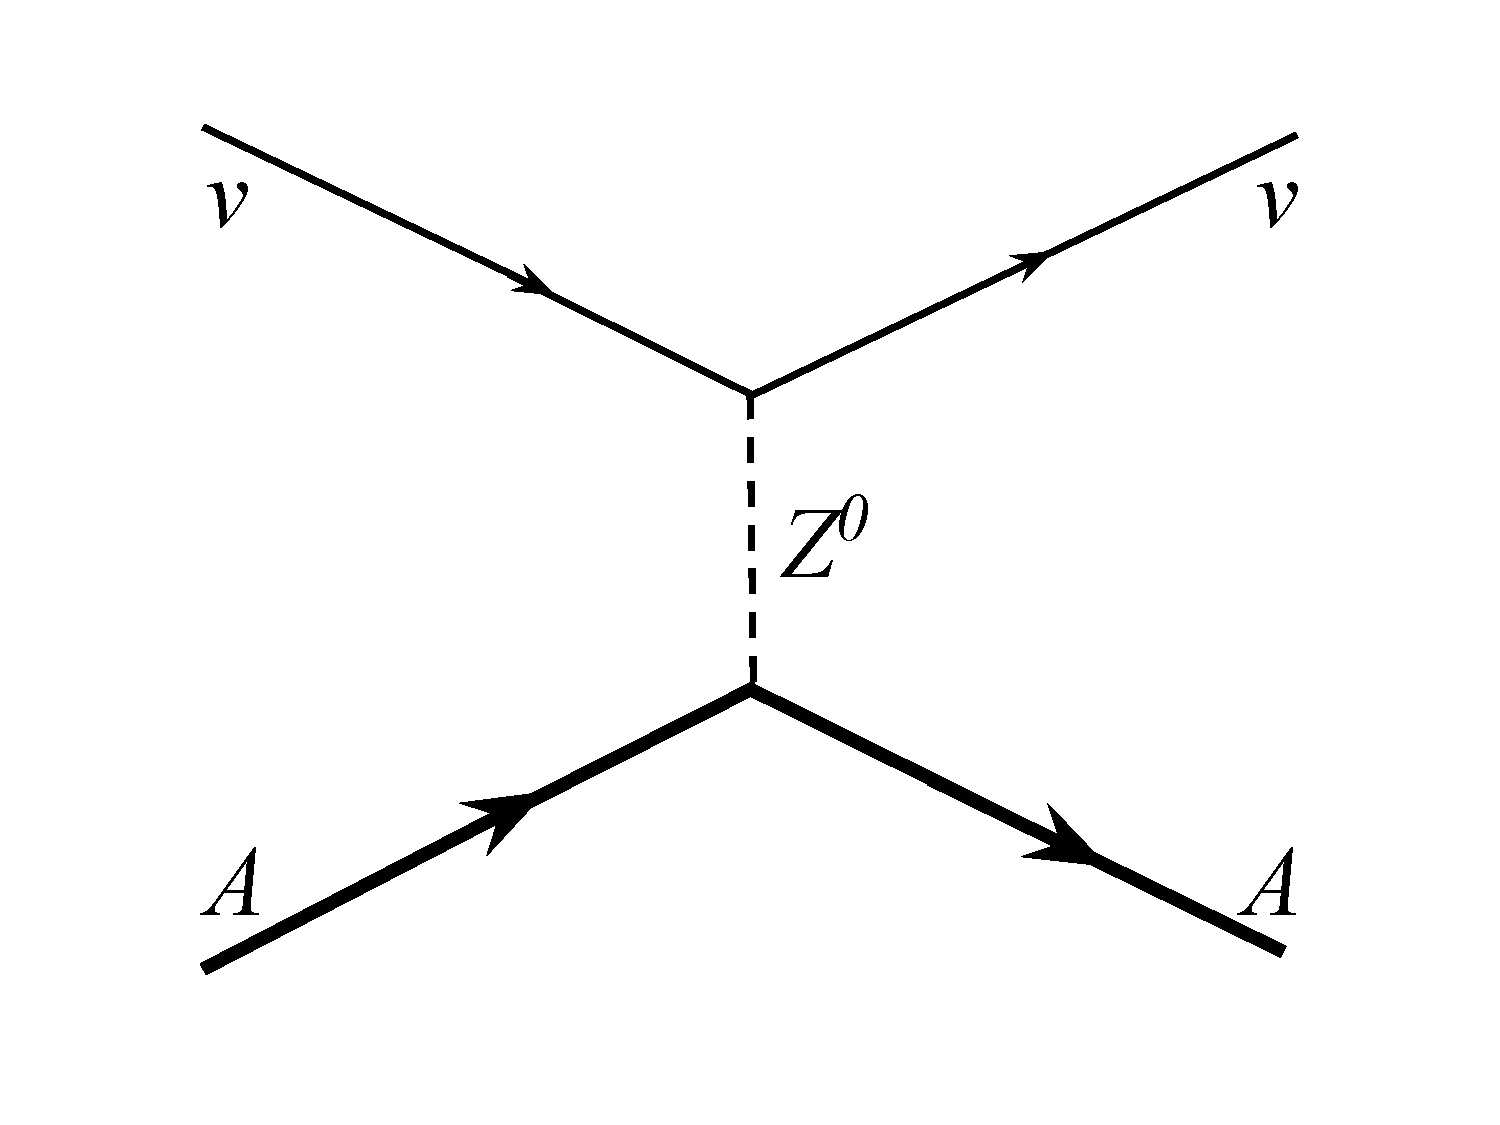
\includegraphics[width=0.6\linewidth]{images/cevns.pdf}}
	\caption{Схема когерентного рассеяния нейтрино на ядре}
	\label{ris:cevns}
\end{figure}
\par Дифференциальное сечение процесса представляется формулой \cite{cevns1, Lindner2017}:
	
\begin{equation}
\frac{d\sigma}{dE_r} = \frac{G_f^2}{4\pi} Q_w^2M\left(1-\frac{ME_r}{2E_\nu}\right)F^2(Q^2),
\end{equation}\\
	
	где $G_f$ --- константа Ферми;
	$Q_w=N-(1-4\sin^{2}\theta_w)Z$ --- слабый заряд для ядра с числом нуклонов $N$ и зарядом ядра $Z$;
	$F(Q^2)$ --- форм-фактор;
	$\theta_w$ --- угол смешивания слабого взаимодействия (угол Вайнберга).
	Используя значение угла можно показать, что сечение взаимодействия
	 $\sim N^2$:\\
	 
	$\sin^2(Q_w)\approx 0.22$ $\to Q_w\sim N \to \sigma \sim N^2$\\
	
	Полное сечение процесса приближённо равно:\\
	
	$\sigma \approx 0.4\cdot10^{-44}  N^2$(E$_\nu^2)$см$^{2}$/МэВ. \\
	\par
	Процесс УКРН имеет место при энергии нейтрино менее 50 МэВ, когда длина волны де Бройля для нейтрино не превосходит размеры ядра, и взаимодействие идет когерентно.
	Отметим, максимальная энергия ядра отдачи равна
\begin{equation}
    T_{max} = \frac{2E_{\nu}^{2}}{M+2E_{\nu}},
    \label{Tmax}
\end{equation}
то есть для большинства элементов энергия ядра отдачи очень мала --- порядка единиц-десятков кэВ на ядро. Таким образом возникают серьезные экспериментальные трудности при регистрации подобных процессов.

Впервые процесс УКРН был зарегистрирован коллаборацией COHERENT в 2017 году на детекторе CsI[Na]~\cite{COHERENT:2017ipa}. Через несколько лет успех коллаборации был повторен и процесс был зарегистрирован на ядрах аргона \cite{PhysRevLett.126.012002}. На данный момент в мире существует более 10 экспериментов по исследованию УКРН. Среди них есть эксперименты как на ускорителях \cite{COHERENT:2018gft}, так и на реакторах \cite{Belov_2015, Aguilar-Arevalo_2016, ricochet, Buck_2020, Singh:2016glu, Strauss_2020, Chaudhuri:2022pqk}. 

\textbf{Раздел 1.2} посвящен двухфазному методу регистрации частиц. В 1970 году Б.А. Долгошеиным был предложен~\cite{Dolgoshein} метод, основанный на использовании двух фаз рабочего вещества. Схема работы метода изображена на рисунке \ref{img:twophase}.
\begin{figure}[h]
	\center{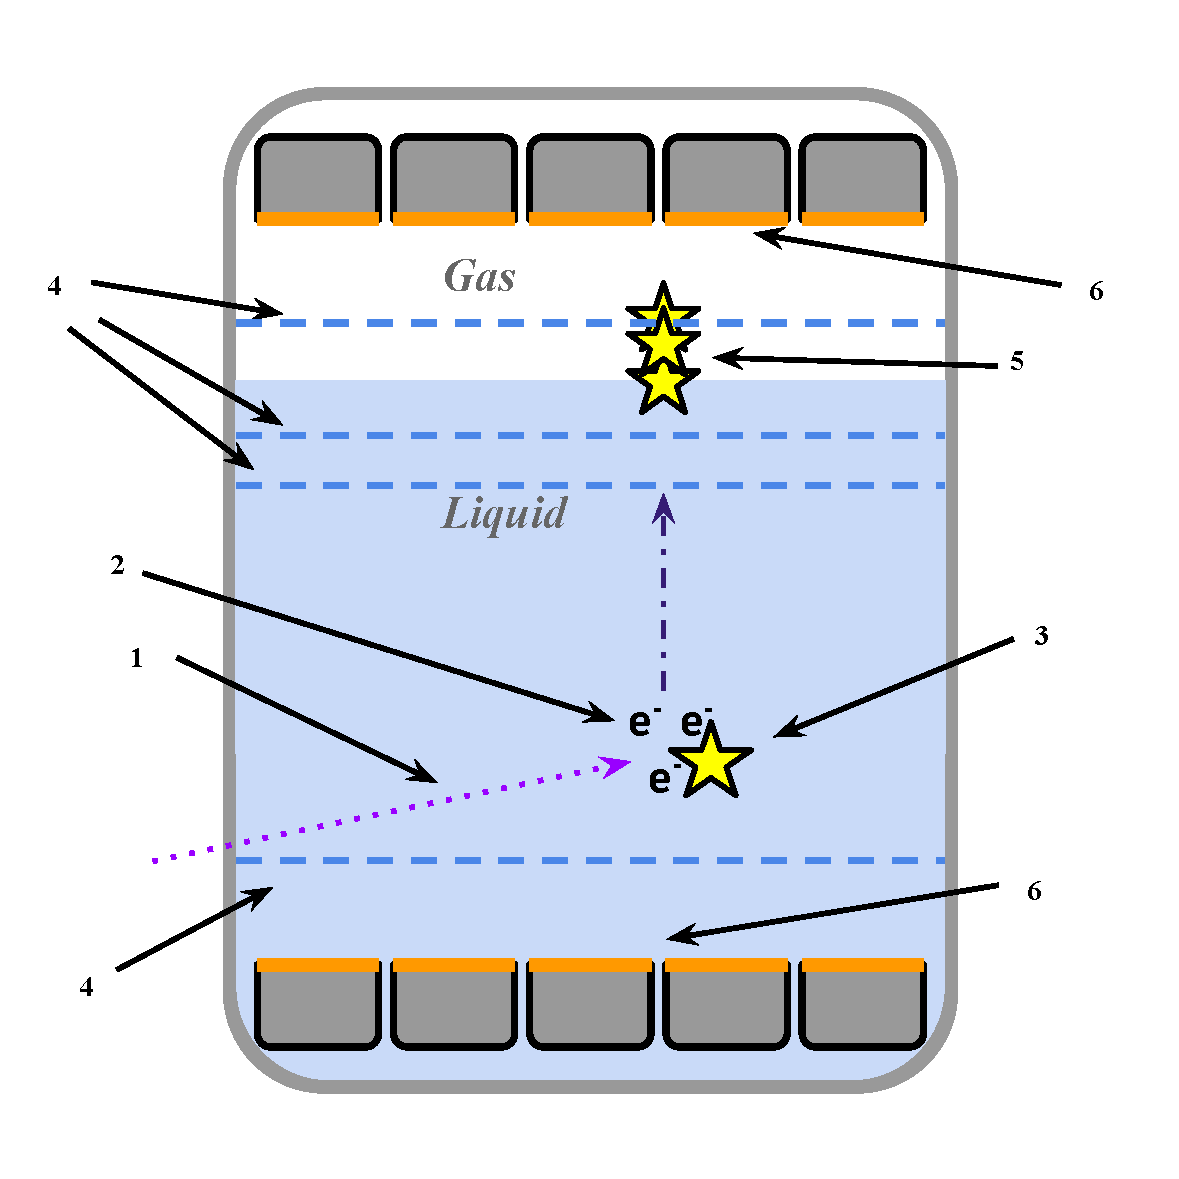
\includegraphics[width=0.7\linewidth]{images/twophasedetector.pdf}}
	\caption[Схема работы двухфазного детектора.] {Схема работы двухфазного детектора. 1 -- трек ионизирующей частицы; 2 -- электроны ионизации, возникшие в результате взаимодействия; 3 -- вспышка сцинтилляции (S1), возникшая в результате взаимодействия; 4 -- электроды-сетки, создающие напряжение; 5 -- электролюминесценция (S2) в электролюминесцентном зазоре; 6 -- матрицы из фотоумножителей}
	\label{img:twophase}
\end{figure}

Двухфазный метод регистрации частиц на данный момент широко используется в экспериментах по поиску темной материи~\cite{BOLOZDYNYA2015405}. Отличительной чертой всех экспериментов по исследованию темной материи явлется расположение глубоко под землей. Толща породы обеспечивала естественное экранирование от космических лучей. Детектор РЭД-100 раполагался на поверхности Земли, что потребовало модификации двухфазного метода регистрации с учетом повышенного фона от космических мюонов. 

\underline{\textbf{Вторая глава}} полностью посвящена эксперименту РЭД-100. В 2021-22 гг. на реакторе четвертого энергоблока Калининской АЭС был поставлен эксперимент РЭД-100 по исследованию УКРН ~\cite{The_RED100_Experiment}. Это один из немногих экспериментов, поставленных на промышленном реакторе. РЭД-100 был создан прицельно для измерения УКРН. Постановке эксперимента на Калининской АЭС предшествовал длительный подготовительный процесс в ЛЭЯФ НИЯУ МИФИ, включавший в себя наладку оборудования и инженерные запуски. 

\textbf{Раздел 2.1} посвящен устройству детектора РЭД-100. Схема детектора РЭД-100 приведена на рисунке \ref{img:detscheme}. Общий вес ксенона в системе РЭД-100 составляет около 200 кг, при этом вес непосредственно рабочего объема, участвующего в регистрации частиц -- 130 кг. В разделе приведено детальное описание газовой и криогенной систем детектора, системы полезадающих электродов-сеток, триггерной системы. 

\begin{figure}[ht!]	\center{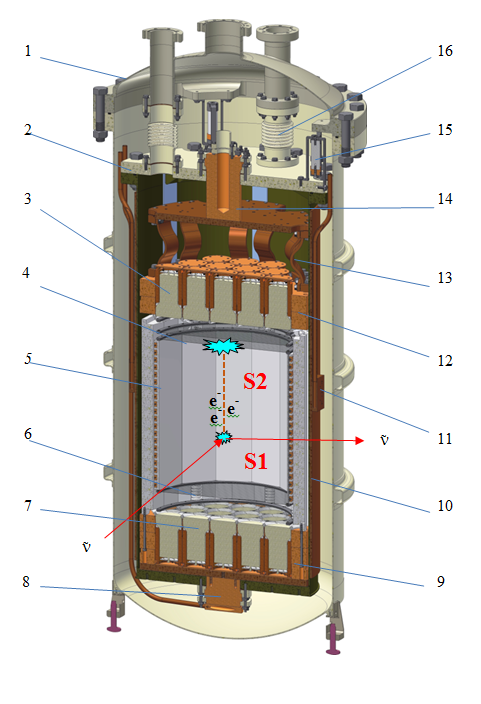
\includegraphics[width=0.5\linewidth]{images/red100.png}}
	\caption[Принцип работы и устройство детектора РЭД-100] {Принцип работы и устройство детектора РЭД-100. 1 --- внешний сосуд титанового криостата, 2 --- внутренний сосуд титанового криостата, 3 --- верхняя матрица из девятнадцати ФЭУ типа Hamamatsu R11410-20, 4 --- сетчатый анод и электронный затвор, 5 --- рабочий объем, окруженный тефлоновым отражателем со встроенными полезадающими электродами, 6 --- сетчатый катод, 7 --- нижняя матрица из девятнадцати ФЭУ, 8 --- нижний центральный теплосъемник с термосифоном, 9 --- медная обойма для нижней матрицы ФЭУ, 10 --- медный кожух холодного сосуда криостата, 11 --- один из двух боковых теплосъемников с термосифонами, 12 --- медная обойма верхней матрицы ФЭУ, 13 --- гибкий тепловой мост, 14 --- верхний центральный теплосъемник с медным диском, на котором конденсируется ксенон, 15 --- теплоизолирующий подвес, 16 --- сильфонная тепловая развязка для вывода кабелей; $e^-$ --- электроны ионизации, $\overline{\nu}$ --- антинейтрино, передающее энергию ядру отдачи, S1 --- сцинтилляционная вспышка, S2 --- электролюминесцентная вспышка.}
	\label{img:detscheme}
\end{figure}

Кроме того, в разделе описаны методы калибровки детектора РЭД-100, такие как:
\begin{itemize}
    \item LED-калибровка
    \item SE-данные (SE -- single electron)
    \item мюонные данные
    \item измерения с гамма-источниками
\end{itemize}
Также в разделе приводится описание основных источников внешнего и внутреннего фона в детекторе. В заключении раздела описан программный пакет RED-Offline, предназначенный для первичной обработки форм сигналов сцинтилляционных детекторов. В первичную обработку входят коррекция наводок, поиск нулевой линии, идентификация и параметризация импульсов. 

\textbf{Раздел 2.2} посвящен конфигурации установки при различных наборах данных. В работе рассматривается инженерный запуск детектора РЭД-100 в 2019 году и физический сеанс на Калининской АЭС в 2021-22 гг. В разделе приведены отличия в типах набираемых данных и конфигурациях пассивной защиты. 
Детектор РЭД-100 на Калининской АЭС располагался в 19 метрах снизу от реактора 4 энергоблока. В в качестве основной пассивной защиты от космических мюонов выступали бетонные перекрытия здания энергоблока. Далее конструкция детектора была помещена в мягкий бак из ПВХ диаметром 5 м, наполненный водой, что обеспечивало пассивную защиту от нейтронов толщиной 60 см. Для защиты от гамма фона вокруг детектора была выстроена конструкция из медных брусков толщиной 5 см. Данные набирались в периоды как с включенным, так и с выключенным реактором для сравнения спектров. 
Всего набирались шесть основных типов данных:
 \begin{enumerate}
     \item LED-калибровки
     \item Мюонные данные
     \item SE-данные
     \item Гамма-фон
     \item Гамма-калибровки
     \item УКРН-подобные данные
 \end{enumerate}
 Типы набранных во время инженерного сеанса в МИФИ данных совпадают с типами данных, набранных на КАЭС, за исключением УКРН-подобных данных. 
 Также в разделе приведены графики нейтронного и гамма фонов, измеренных на протяжении постановки эксперимента на КАЭС при помощи вспомогательных детекторов (NaI[Tl] и Bicron) (рисунок~\ref{img:gammaneutronbckg}).

 \begin{figure}[ht!]
  \begin{minipage}[ht]{0.49\linewidth}
    \center{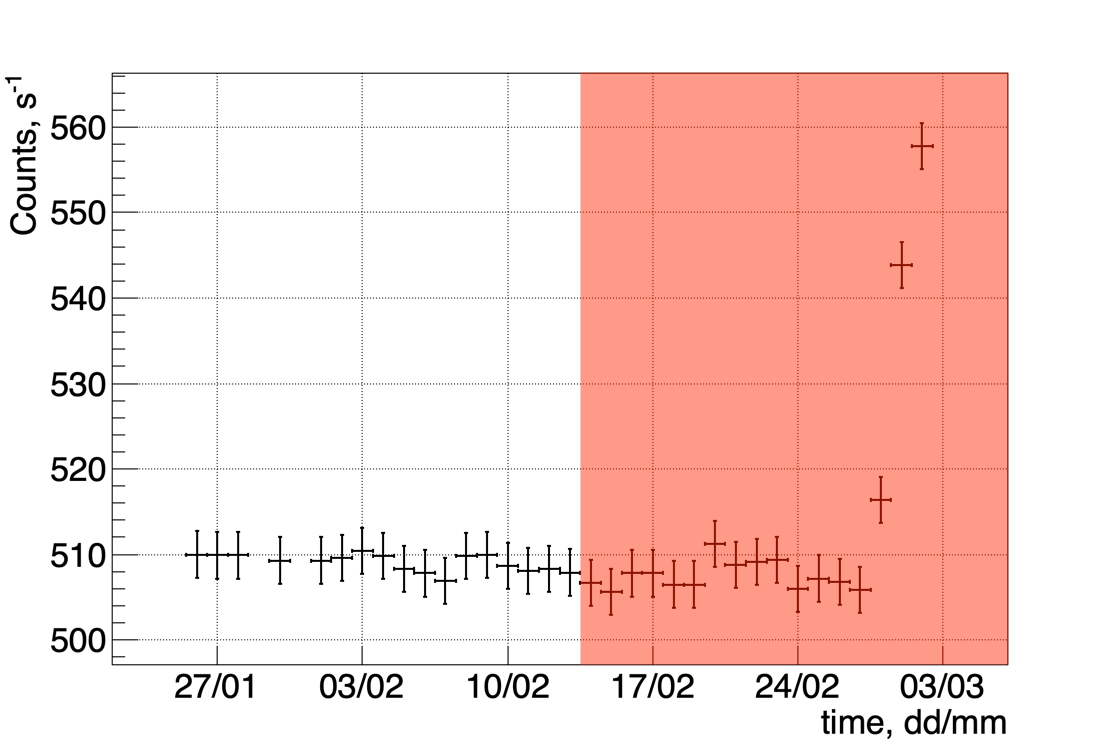
\includegraphics[width=1.0\linewidth]{images/NaI_count_rate_monitoring.png} \\ а)}
  \end{minipage}
  \hfill
  \begin{minipage}[ht]{0.49\linewidth}
    \center{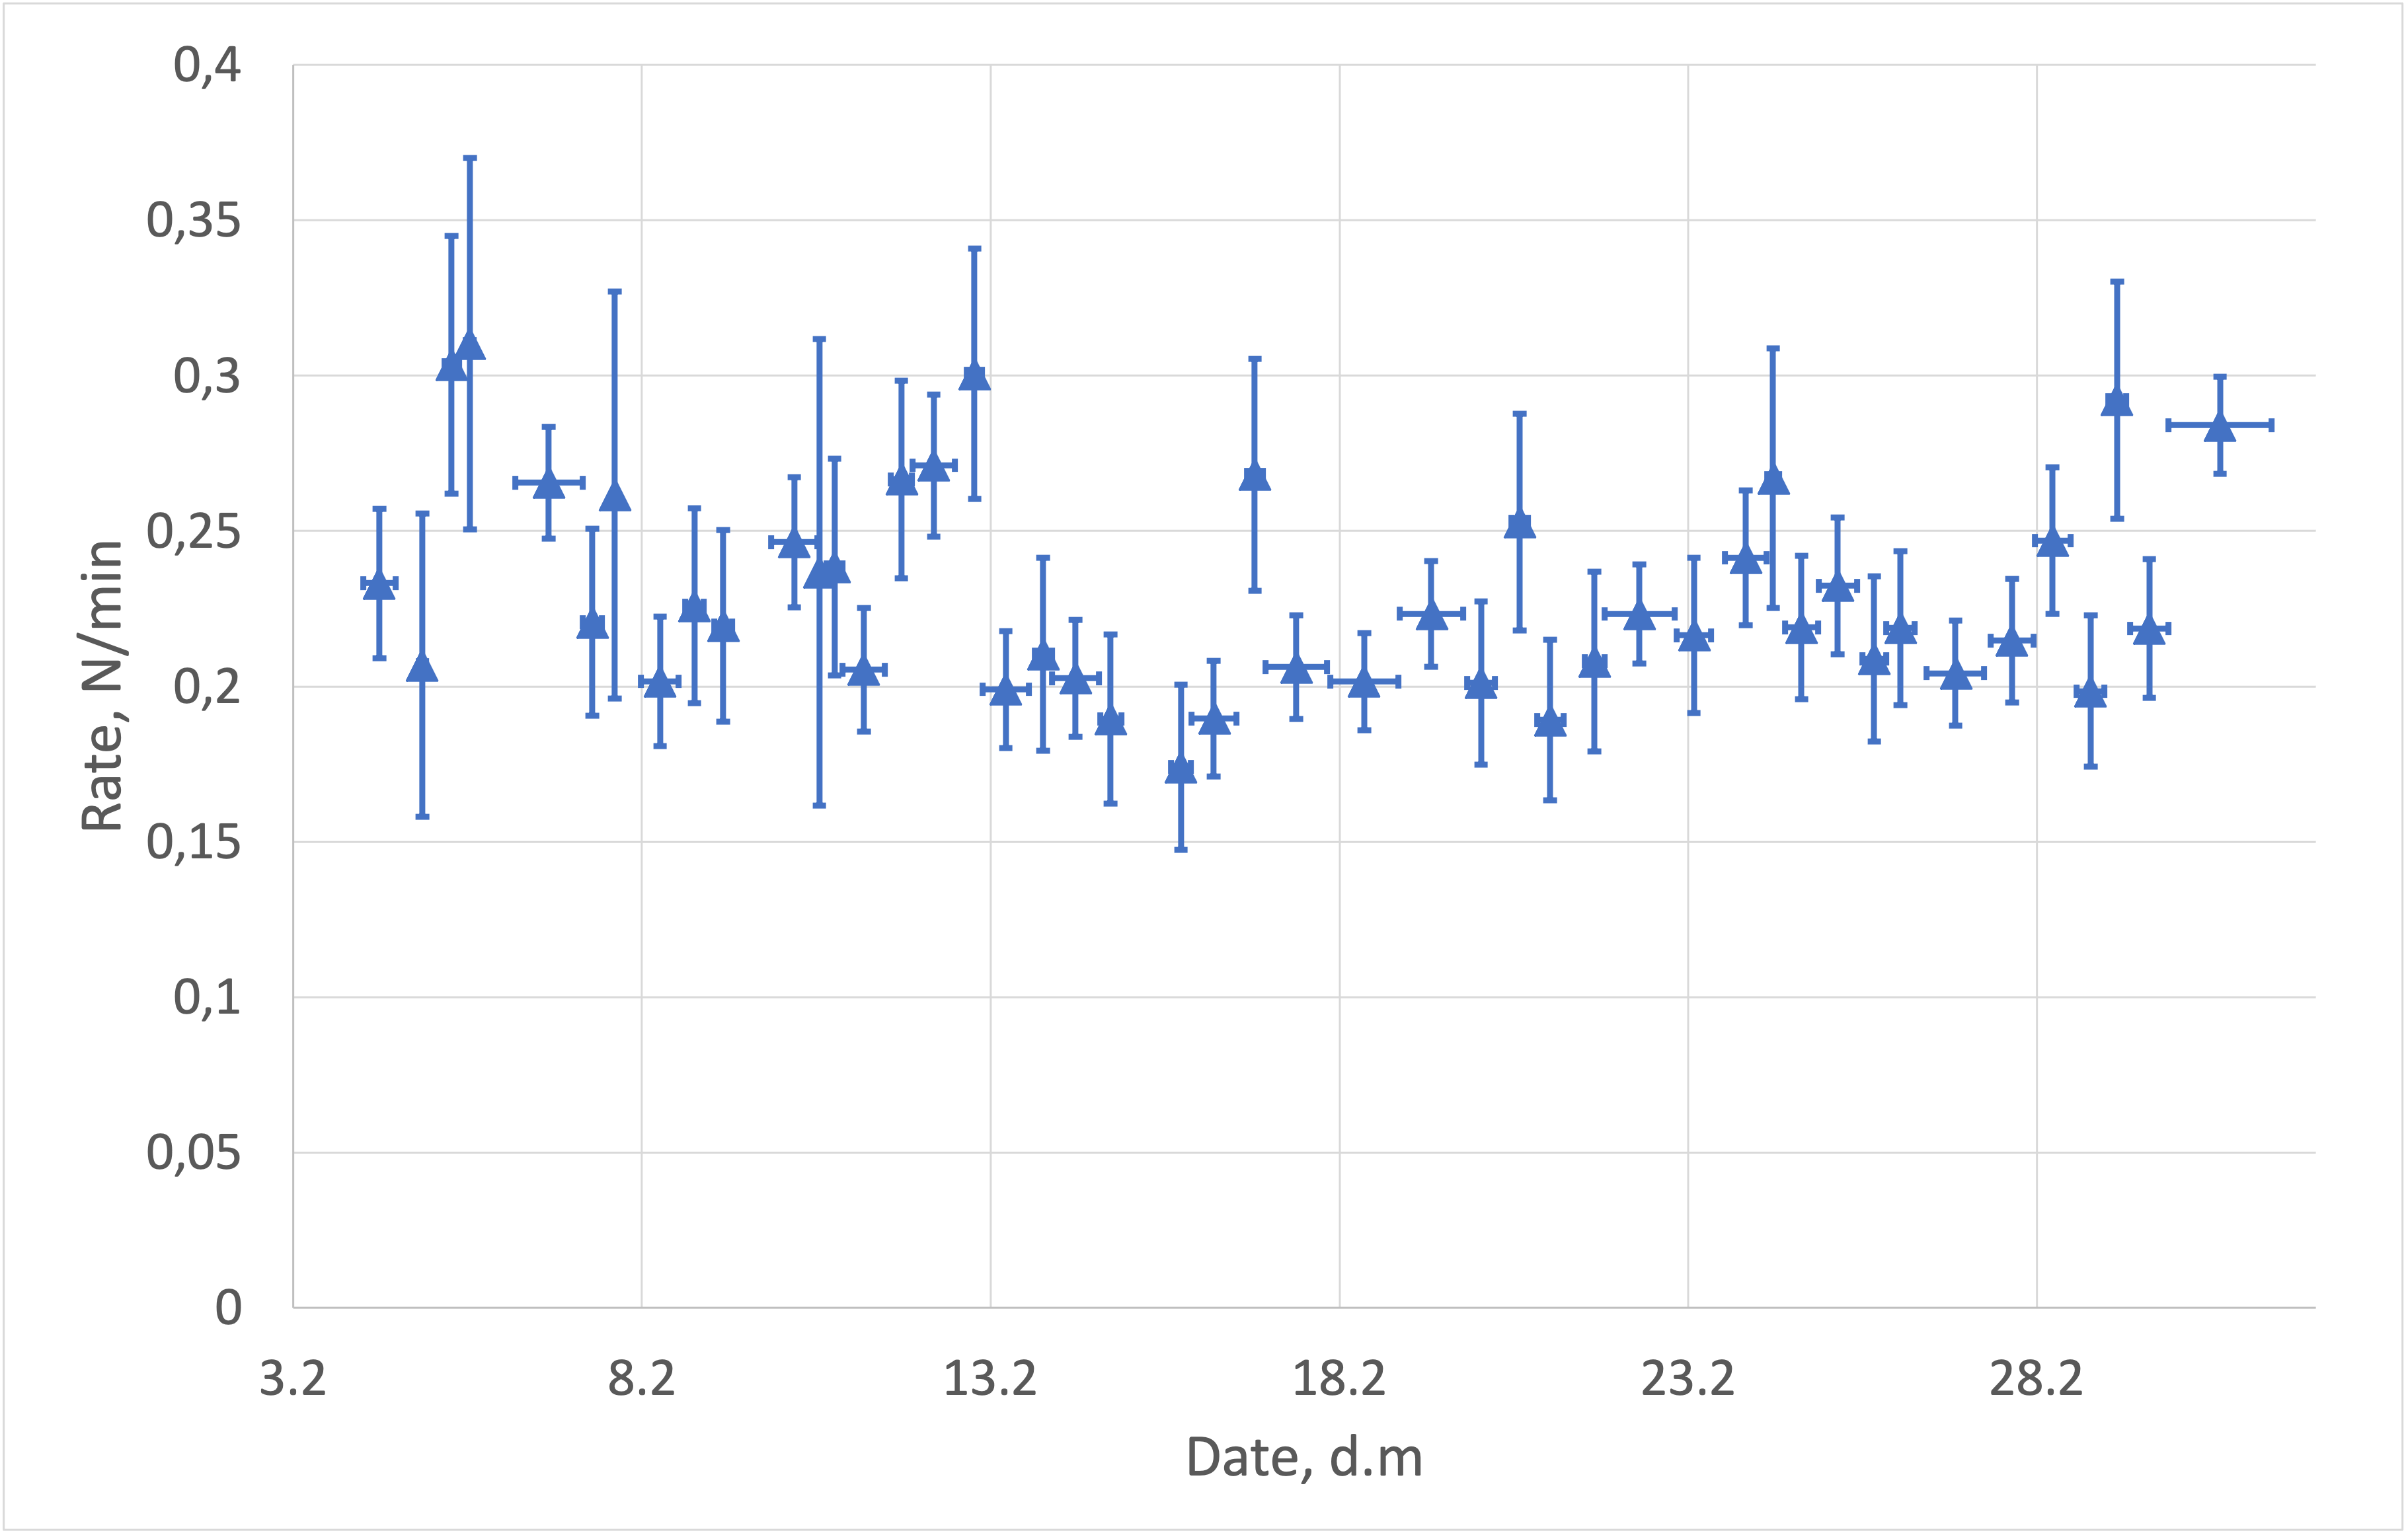
\includegraphics[width=1.0\linewidth]{images/neutrons_rate.png} \\ б)}
  \end{minipage}
  \caption[Графики изменения гамма и нейтронного фонов.]{а) График изменения гамма-фона (измерения суммировались за каждые 3 часа набора данных). б) График изменения нейтронного фона}
  \label{img:gammaneutronbckg}  
\end{figure}

 \textbf{Раздел 2.3} посвящен моделированию детектора РЭД-100. Приведено описание моделей детектора в трех программных пакетах (GEANT4, NEST, ANTS-2), а также описание моделирования временных разверток сигналов. 

 \underline{\textbf{Третья глава}} посвящена анализу калибровочных данных детектора РЭД-100.  
 
 \textbf{Раздел 3.1} посвящен калибровке мюонами. При дрейфе в ксеноне электроны ионизации претерпевают потери, связанные с захватом их примесями. Как известно, процесс таких потерь описывается экспоненциальной функцией. Для измерения времени жизни мюонные сигналы, записанные в специальном режиме работы детектора, фитировались функцией $ f(t) = A\cdot exp(-\frac{t}{\tau})$, где $\tau$ -- среднее времени
жизни электронов до захвата $\tau$, за которое количество дрейфующих электронов ионизации уменьшается в e раз. Пример усредненного сигнала и его фитирования приведен на рисунке \ref{img:muonsignal}. Усреднение сигнала проводилось путем суммирования большого количества одиночных сигналов.
\begin{figure}[ht!]	\center{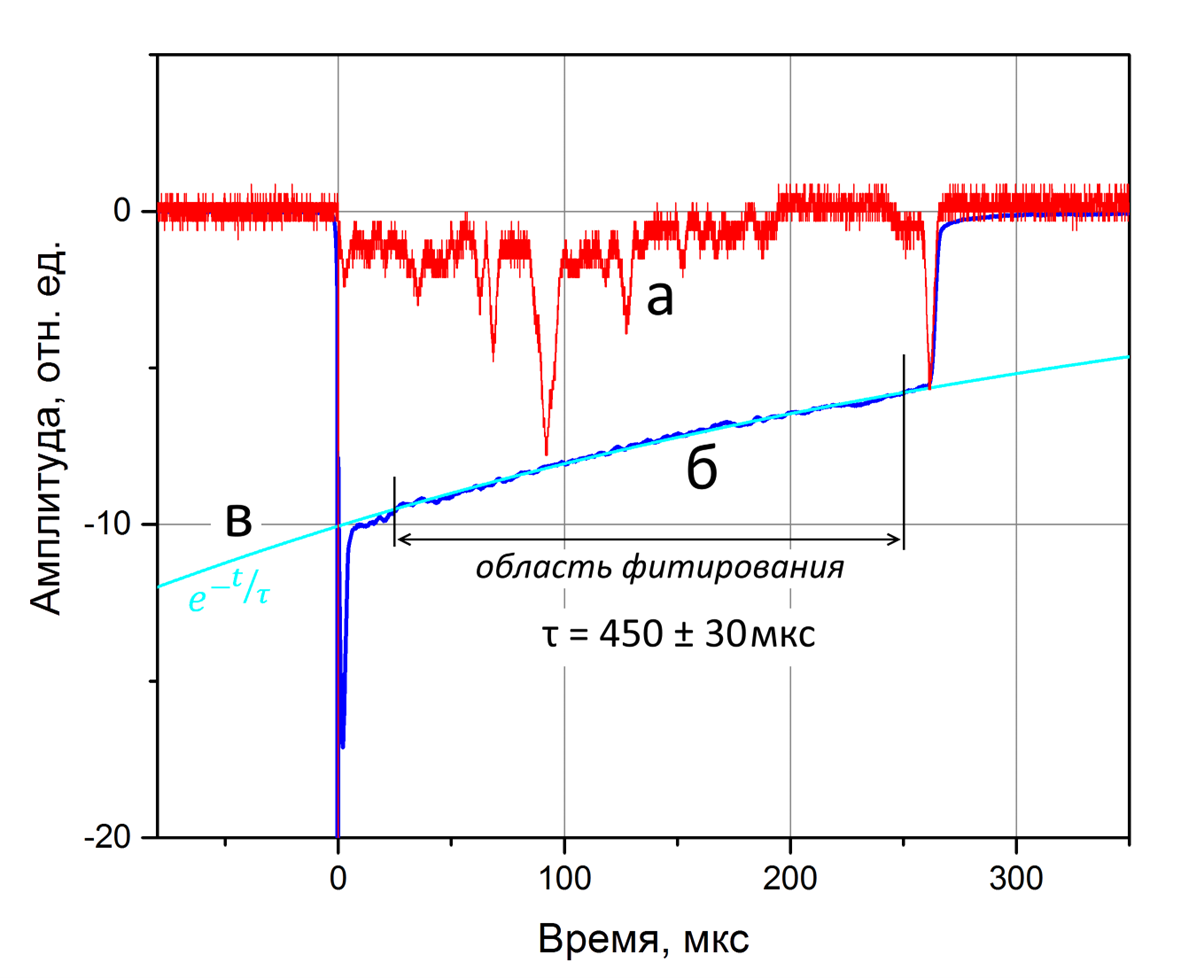
\includegraphics[width=0.8\linewidth]{images/Graph41_labels.png}}
	\caption[Пример определения времени жизни электронов ионизации до захвата электроотрицательными примесями в жидком ксеноне.]{а) — типичный мюонный сигнал, б) — сигнал, усреднённый по 10 000 событий, в — экспоненциально спадающая функция, аппроксимирующая «ступеньку» усреднённого сигнала.}
	\label{img:muonsignal}
\end{figure}

Эволюция времени жизни в течение сеанса показана
на рисунках \ref{img:lt2019}, \ref{img:lt2022}

\begin{figure}[ht!]	\center{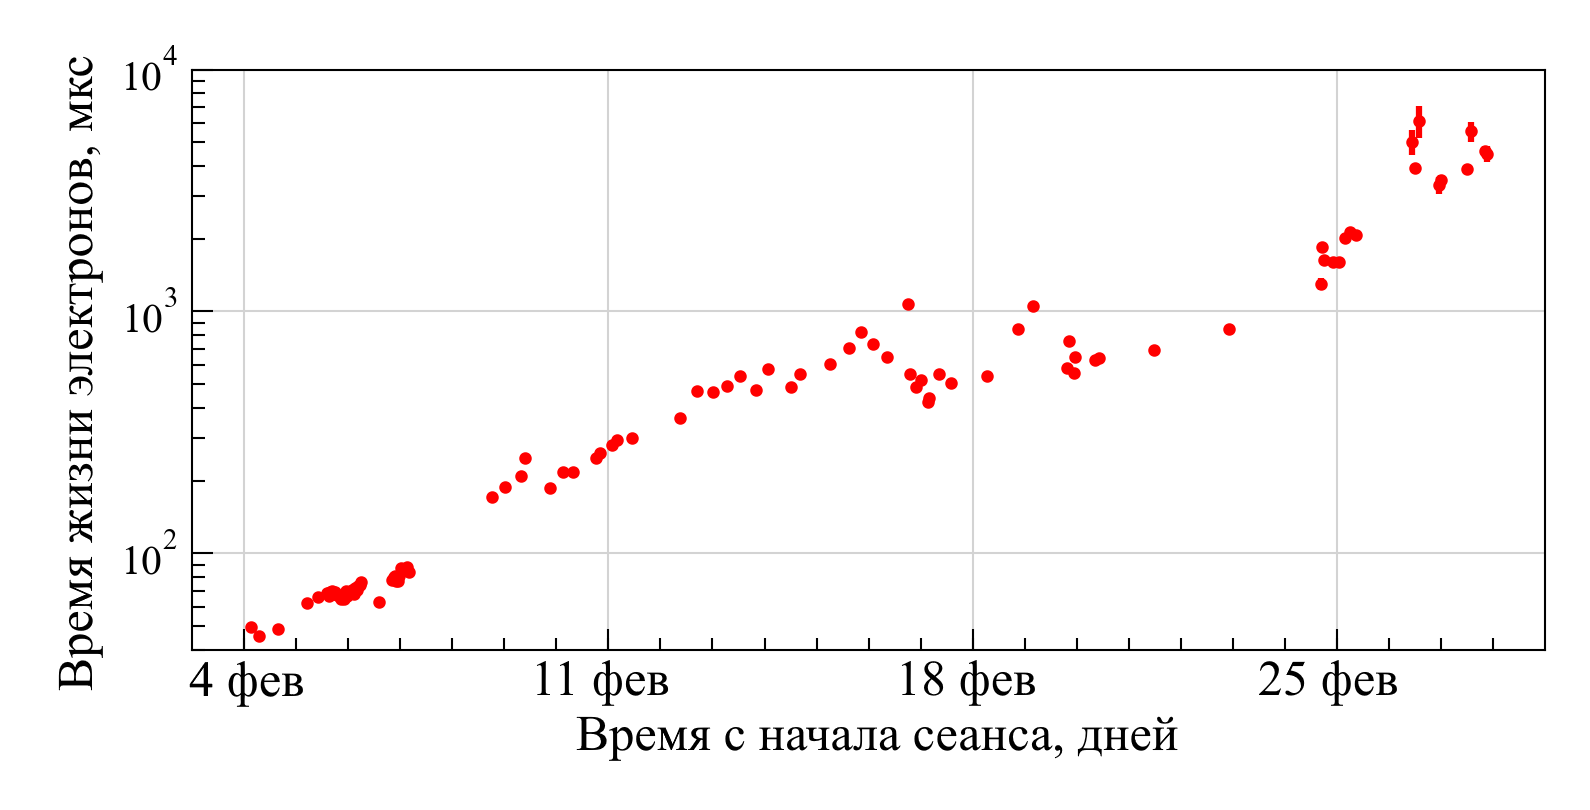
\includegraphics[width=0.8\linewidth]{images/RED100. Graph. e_lifetime_2019_published_RU.png}}
	\caption{Динамика изменения времени жизни электронов в детекторе РЭД-100 в течение инженерного сеанса 2019 года}
	\label{img:lt2019}
\end{figure}

\begin{figure}[ht!]	\center{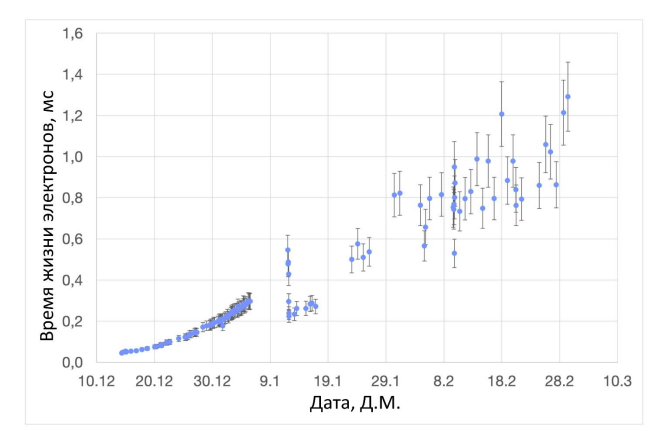
\includegraphics[width=0.8\linewidth]{images/lifetime2022.png}}
	\caption{Динамика изменения времени жизни электронов в детекторе РЭД-100 в течение сеанса на КАЭС 2022 года}
	\label{img:lt2022}
\end{figure}

В \textbf{разделе 3.2} описывается LED-калибровка, необходимая для определения среднего заряда SPE (single photo-electron) для каждого ФЭУ. После обработки данных пакетом REDOffline, из обнаруженных импульсов отбирались импульсы с амплитудой и длительностью больше пороговых. Далее распределение площадей отобранных импульсов фитировалось суммой экспоненциальной функции и распределения Гаусса, и исходя из параметров полученного распределения Гаусса вычислялся средний заряд SPE для каждого ФЭУ. Далее полученные значения использовались для перевода площадей импульсов из В$\cdot$c в единицы SPE.

\textbf{Раздел 3.3} посвящен анализу измерений с гамма-источниками. В 2019 году в качестве калибровочных источников использовались $^{60}$Co и $^{22}$Na, в 2021-22 -- $^{60}$Co и $^{137}$Cs. 

Гамма-кванты дают световыход в детекторе, достаточно большой для того, чтобы в каждом ФЭУ был ощутимый световой сигнал. Поэтому для анализа применяется суммарная форма сигнала, в которой импульсы от физических сигналов в разных ФЭУ будут складываться, а совпадений случайных импульсов с таковыми в других ФЭУ не будет. В разделе описан алгоритм кластеризации, позволяющий отбирать S1 и S2, соответствующие подобным событиям.

После кластеризации на события накладывались дополнительные отборы по глубине и по количеству S1 и S2 в каждом событии (строго по одной вспышке каждого вида). В разделе подробно описаны методы восстановления координат S2 в плоскости XY и энергии событий на основе LRF (light response functions). Кроме того, описан итеративный процесс получения данных функций. Восстановление координат и энергии позволяет существенно уменьшить зависимость светосбора от радиуса. 

В двухфазных детекторах присутствует антикорреляция между S1 и S2, поэтому в качестве энергии рассматривалась линейная комбинация сцинтилляции и электролюминесценции. Также для улучшения соотношения сигнал/шум на события были наложены дополнительные отборы по восстановленному радиусу (175 мм для сеанса в МИФИ и 130 мм для сеанса на КАЭС). Калибровочные графики для двух сеансов набора данных приведены на рисунках~\ref{img:calibplot2019},~\ref{img:calibr2022}, а энергетическое разрешение и положения пиков -- в таблицах~\ref{tab:resolution2019}~и~\ref{tab:resolution2022}. Различия в энергетическом разрешении связаны с различными отборами в двух сеансах и методами фитирования спектров.

\begin{figure}[ht]
\center{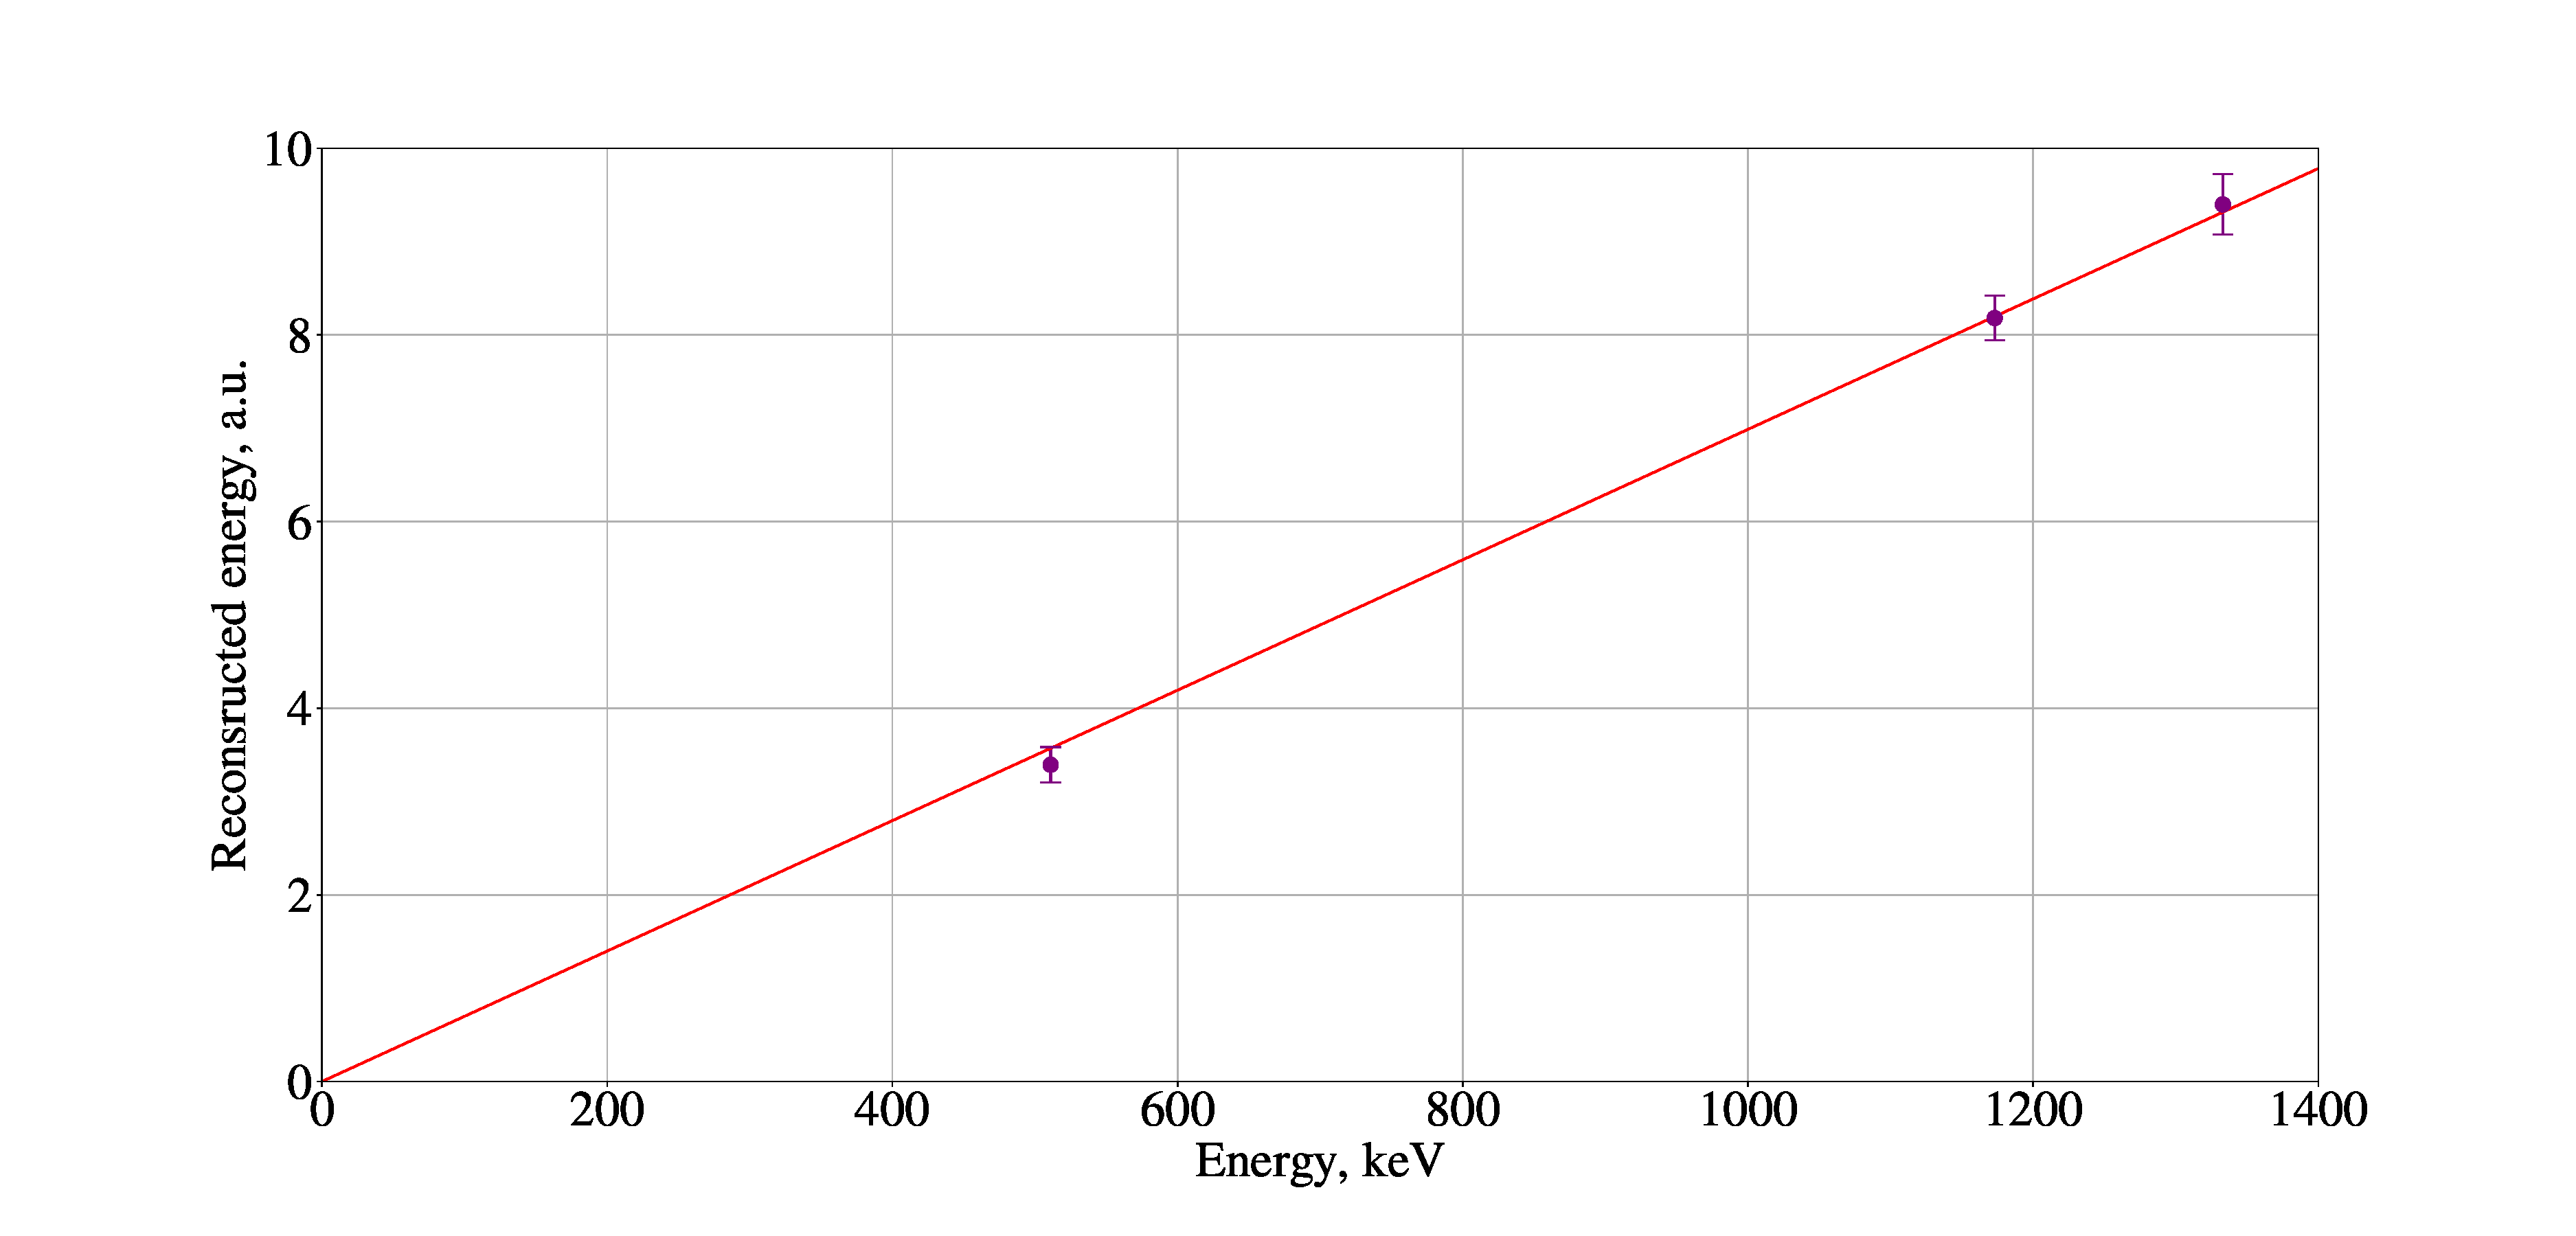
\includegraphics[width=1\linewidth]{images/calibr.pdf}}
  \caption{Калибровочный график для инженерного сеанса 2019 года.}
  \label{img:calibplot2019}  
\end{figure}

\begin{table}[ht]
    \centering
        \caption{Положения пиков и энергетическое разрешение}
\begin{tabular}{|c|c|c|c|}
\hline
    Энергия, кэВ & Положение пика, кэВ & ($\sigma/E$), \% & FWHM/E,  \%\\
    \hline
    511 & 486$\pm$29 & 5.5$\pm$0.1 & 12.9$\pm$0.2\\
    \hline
    1173 & 1171$\pm$34 & 5.4$\pm$0.1 & 12.7$\pm$0.3\\
    \hline
    1333 & 1345$\pm$46 & 4.8$\pm$0.2 & 11.3$\pm$0.4\\
    \hline
\end{tabular}
    \label{tab:resolution2019}
\end{table}

\begin{figure}[ht]
\center{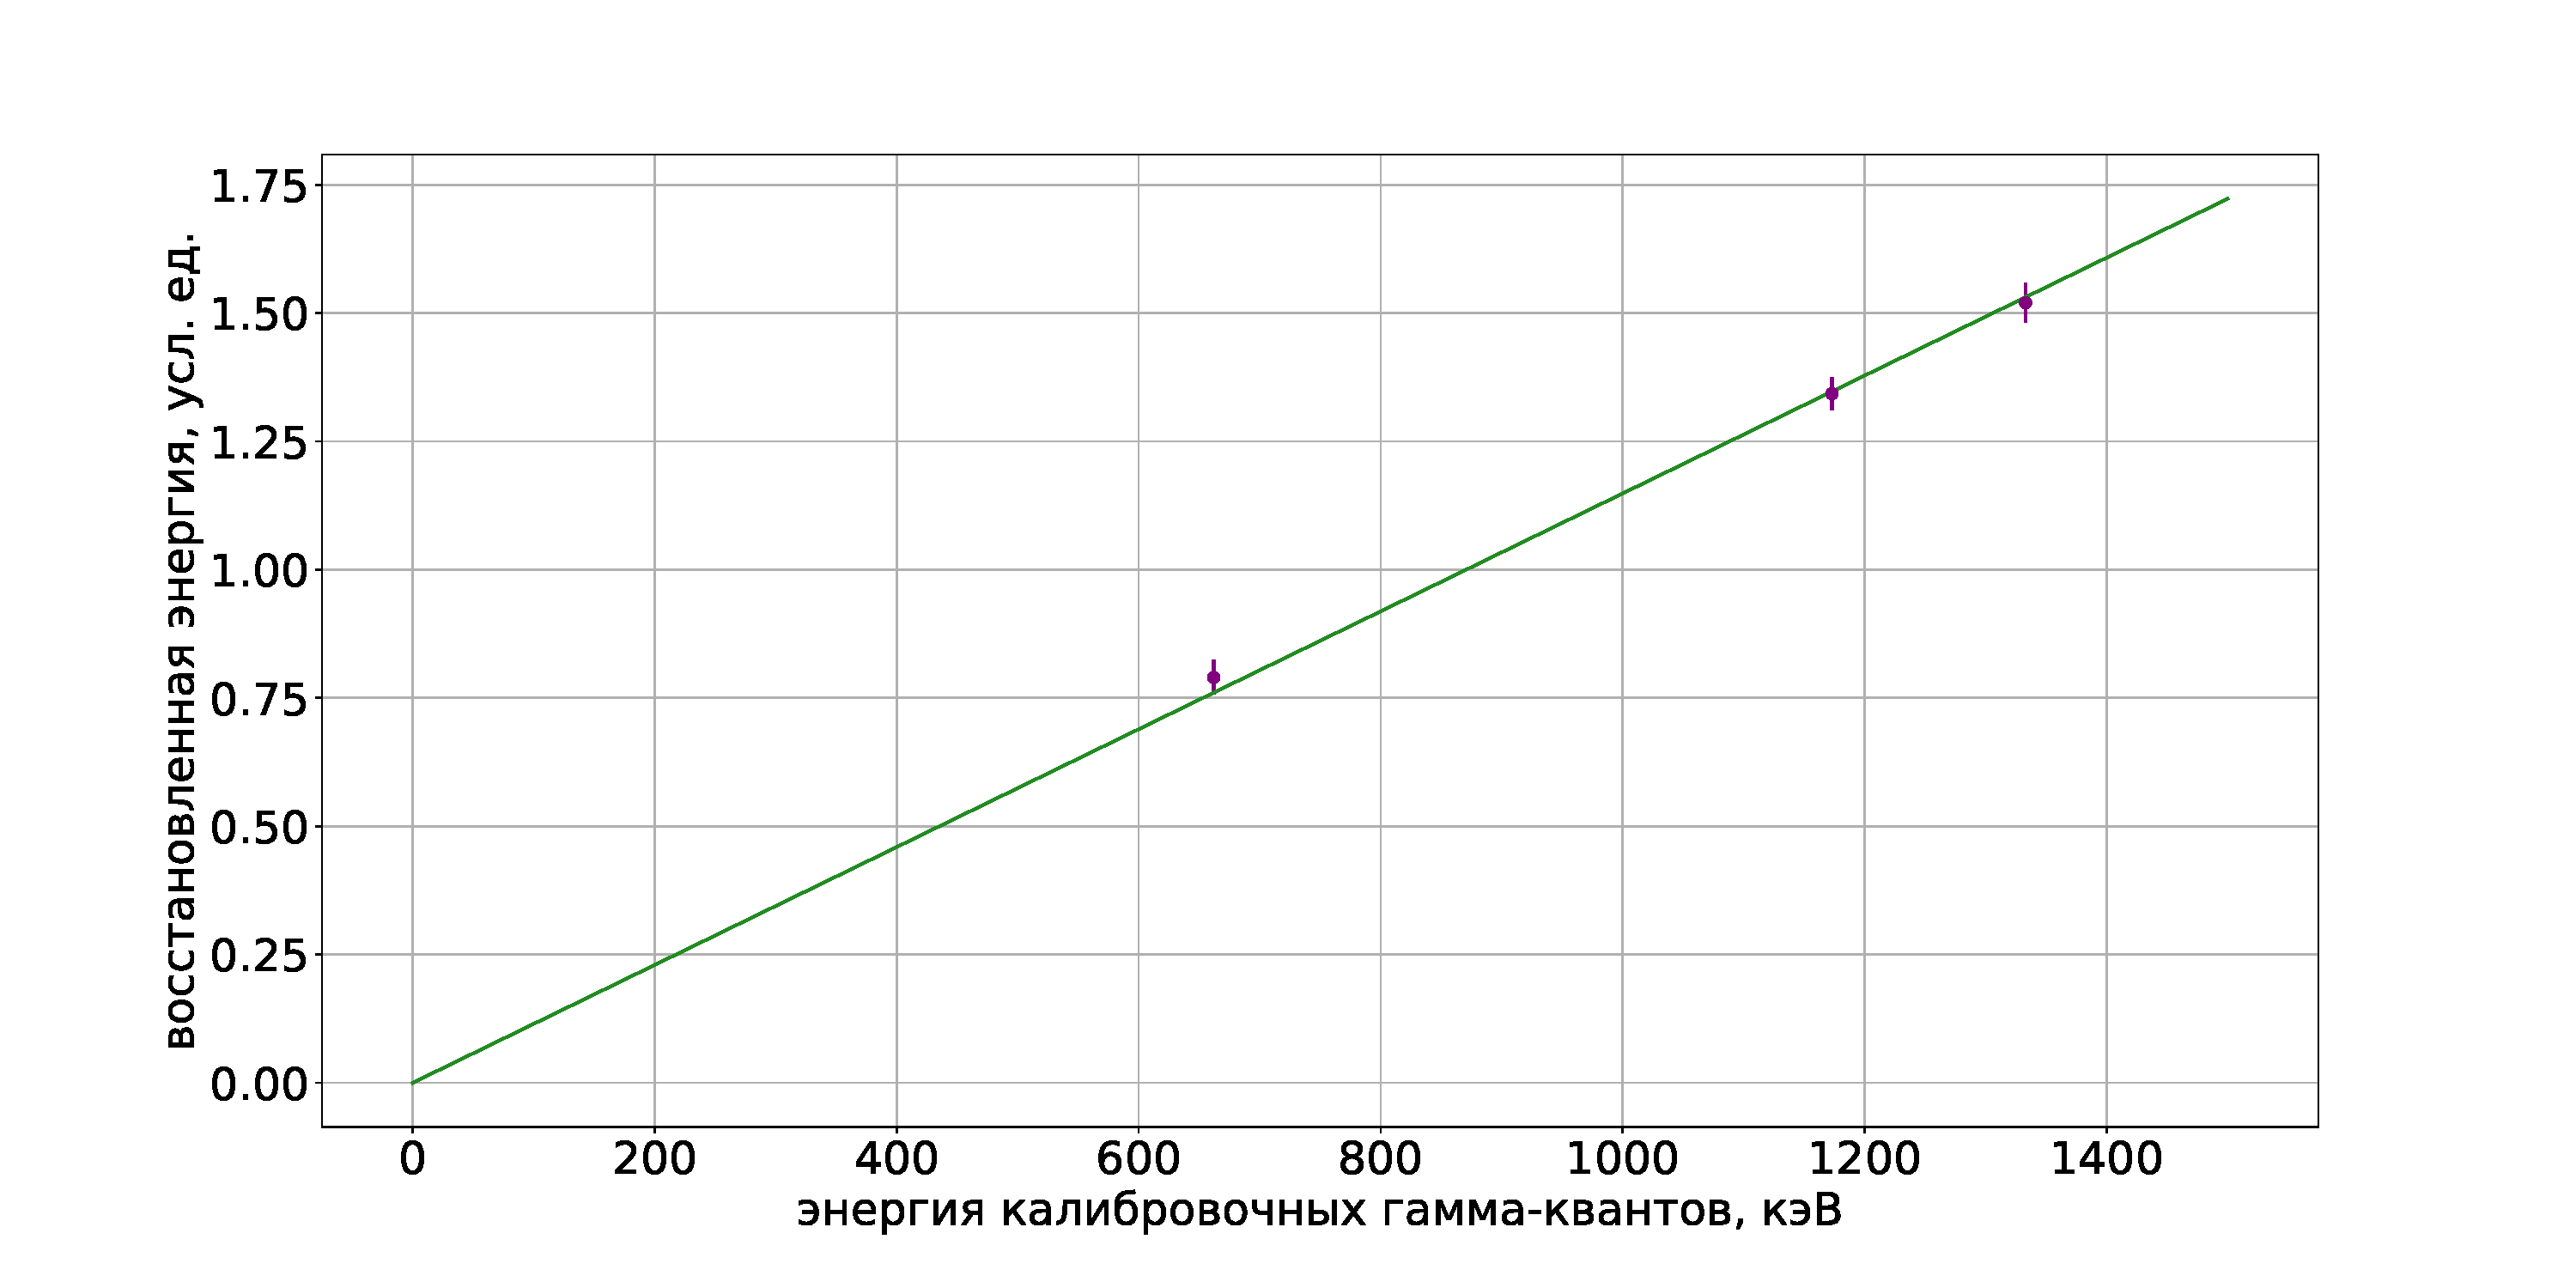
\includegraphics[width=1\linewidth]{images/calibr2022.pdf}}
  \caption{Калибровочный график для сеанса на КАЭС}
  \label{img:calibr2022}  
\end{figure}

\begin{table}[ht]
    \centering
        \caption{Положения пиков и энергетическое разрешение (сеанс на КАЭС)}
\begin{tabular}{|c|c|c|c|}
\hline
    Энергия, кэВ & Положение пика, кэВ & ($\sigma/E$), \% & FWHM/E,  \%\\
    \hline
    662 & 688$\pm$29 & 8.4 & 19.6\\
    \hline
    1173 & 1169$\pm$27 & 3.7 & 8.7\\
    \hline
    1333 & 1323$\pm$33 & 3.9 & 9.2\\
    \hline
\end{tabular}    
\label{tab:resolution2022}
\end{table}

\textbf{Раздел 3.4} посвящен SE-калибровкам. Сигналы от одиночных электронов ионизации представляют собой кластеры из равномерно распределенных по времени внутри кластера однофотоэлектронных импульсов. Как уже было упомянуто, SE-данные предсталяют собой формы сигналов в случайные моменты времени. Данные формы сигналов могут содержать как и искомые сигналы, так и совершенно разные события, а также случайные импульсы. Для отбора кластеров импульсов, соответствующих сигналам от одиночных электронов ионизации был применен следующий алгоритм:
\begin{enumerate}
    \itemОтбирались импульсы с амплитудой больше пороговой. Пороговые значения вычислялись как $\mu-2\sigma$, где $\mu$ и $\sigma$ -- параметры фита однофотоэлектронного спектра в соответствующем канале.
    \itemОтбирались такие последовательности импульсов, чтобы между любыми двумя из них расстояние было не больше $\Delta T$=500~нс. Величина $\Delta T$ подбиралась экспериментально исходя из знания о том, что длительность кластера, соответствующего электролюминесценции, составляет~$\approx$2~мкс. 
\end{enumerate}

Распределение SE-событий по длительности представлено на рисунке~\ref{img:seduration}. Как и во время сеанса на КАЭС, так и во время инженерного сеанса наблюдались события длительностью существенно меньшей, чем средняя длительность электролюминесценции. Данные события на графиках, представленных на рисунке~\ref{img:seduration}, составляют пик слева от основного. Такие "короткие" события возникают, если электролюминесценция происходит с самого края детектора, где электролюминесцентный зазор ограничен кольцом-держателем сетки. Для дальнейшего анализа данные события были отброшены. Границы отбора по длительности показаны на рисунке~\ref{img:seduration} красными линиями. Распределения суммарного светосбора по данным верхней матрицы для SE-данных представлены на рисунке~\ref{img:sespesp}.
\begin{figure}[ht]
  \begin{minipage}[ht]{0.49\linewidth}    \center{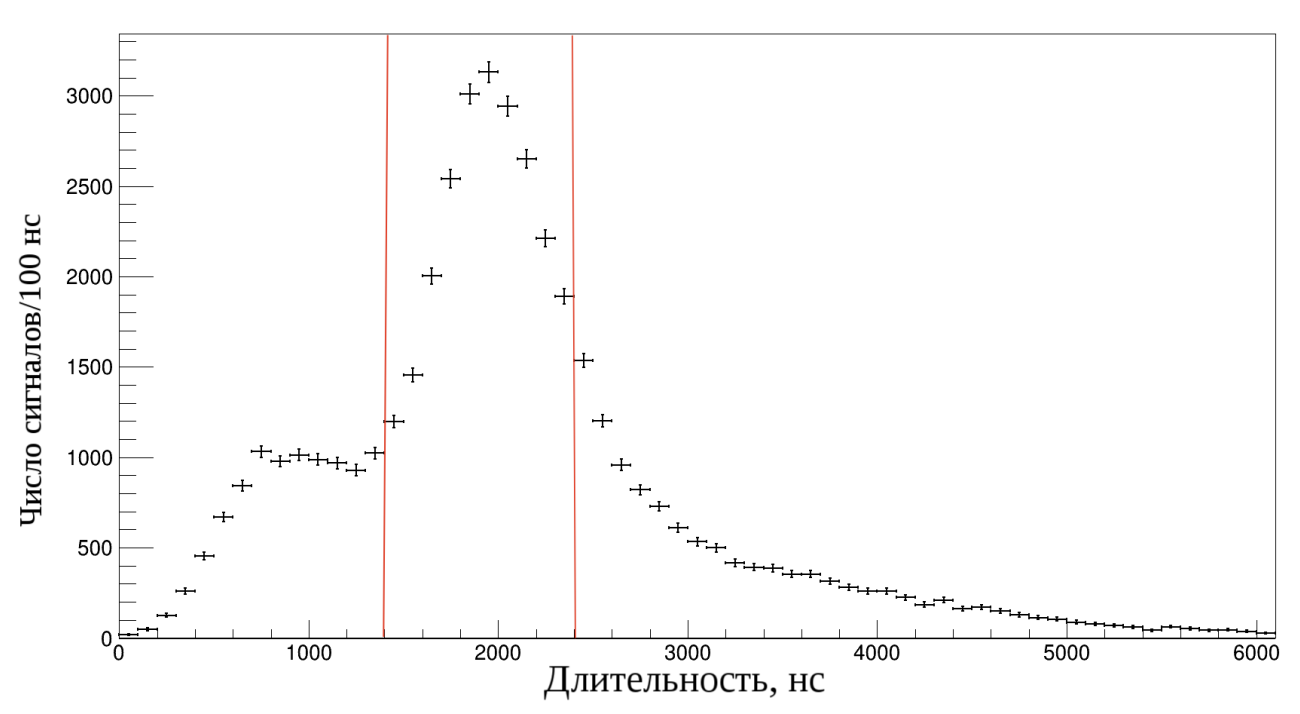
\includegraphics[width=1.0\linewidth]{images/seduration2019.png} \\ а)}
  \end{minipage}
  \hfill
  \begin{minipage}[ht]{0.49\linewidth}  \center{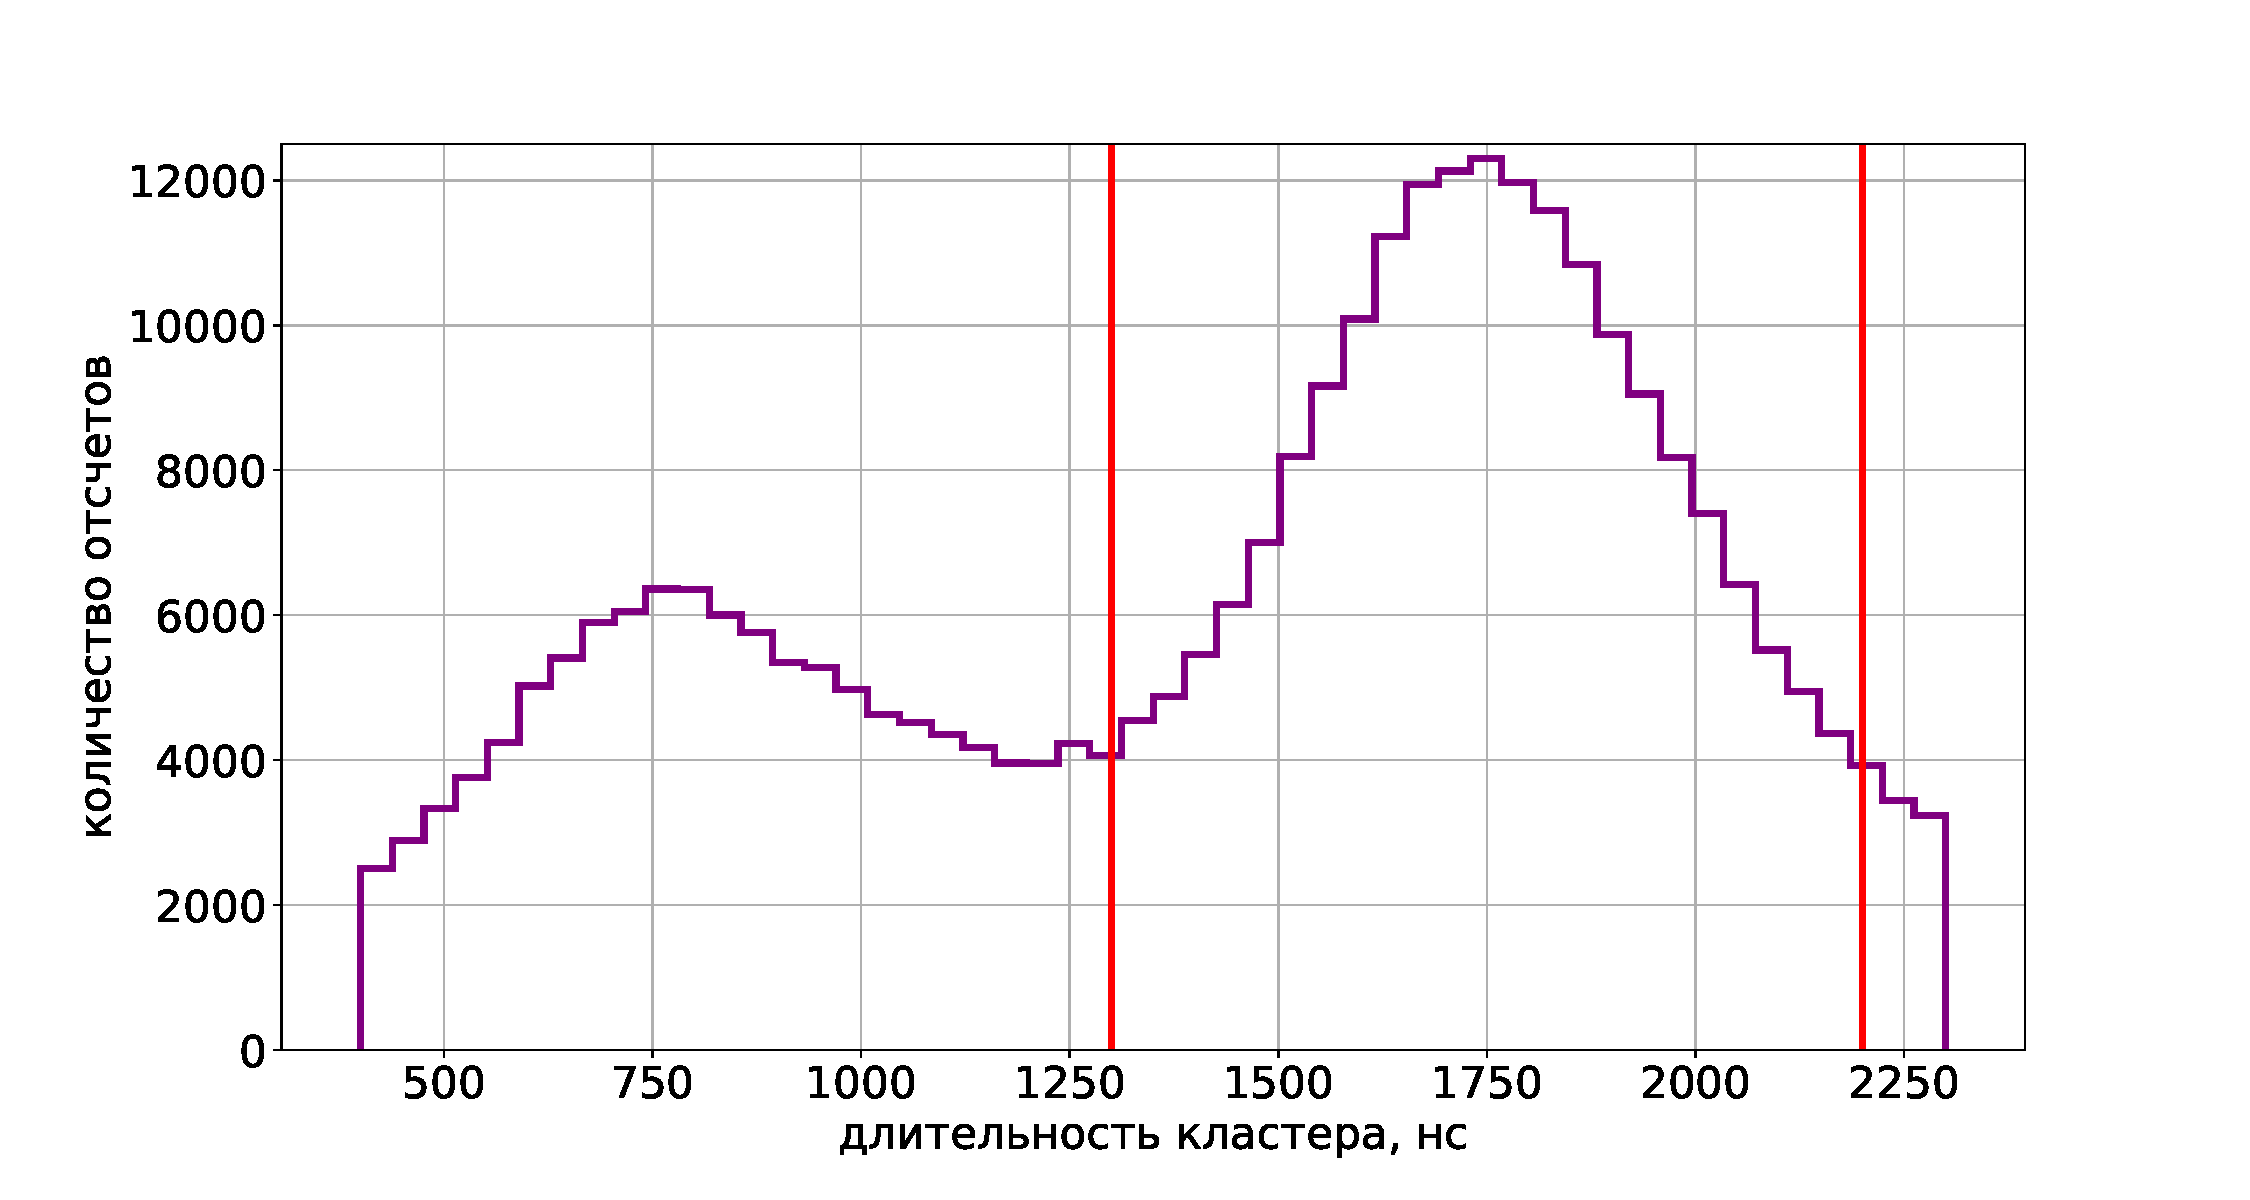
\includegraphics[width=1.0\linewidth]{images/seduration2022.pdf} \\ б)}
  \end{minipage}
  \caption{Распределение событий по длительности для инженерного сеанса (слева) и сеанса на КАЭС (справа)}
  \label{img:seduration}  
\end{figure}

\begin{figure}[ht]
  \begin{minipage}[ht]{0.49\linewidth}    \center{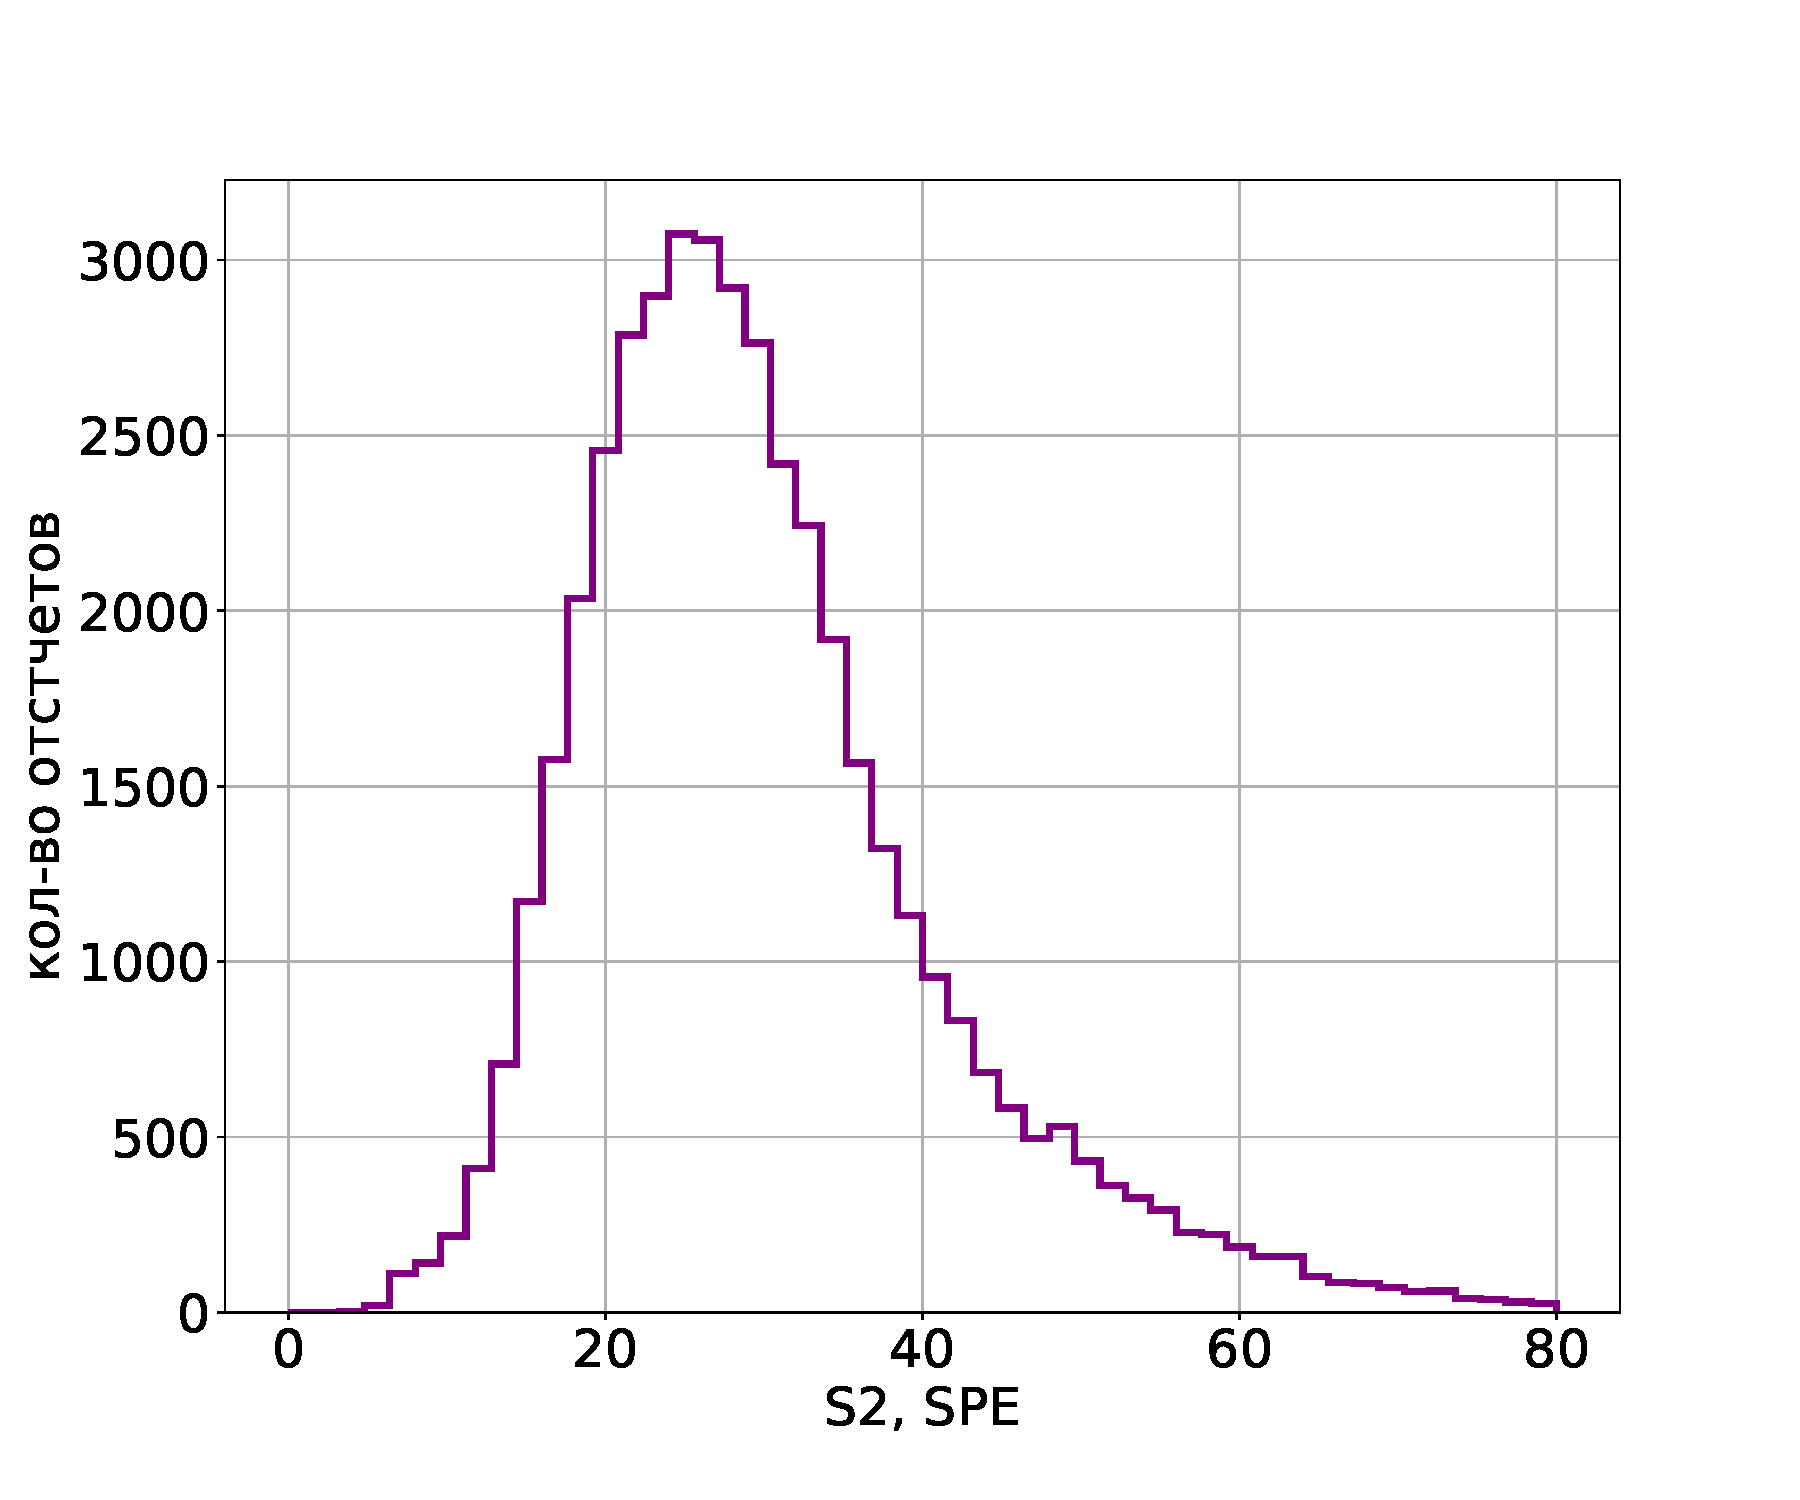
\includegraphics[width=1.0\linewidth]{images/se2019sp.pdf} \\ а)}
  \end{minipage}
  \hfill
  \begin{minipage}[ht]{0.49\linewidth}  \center{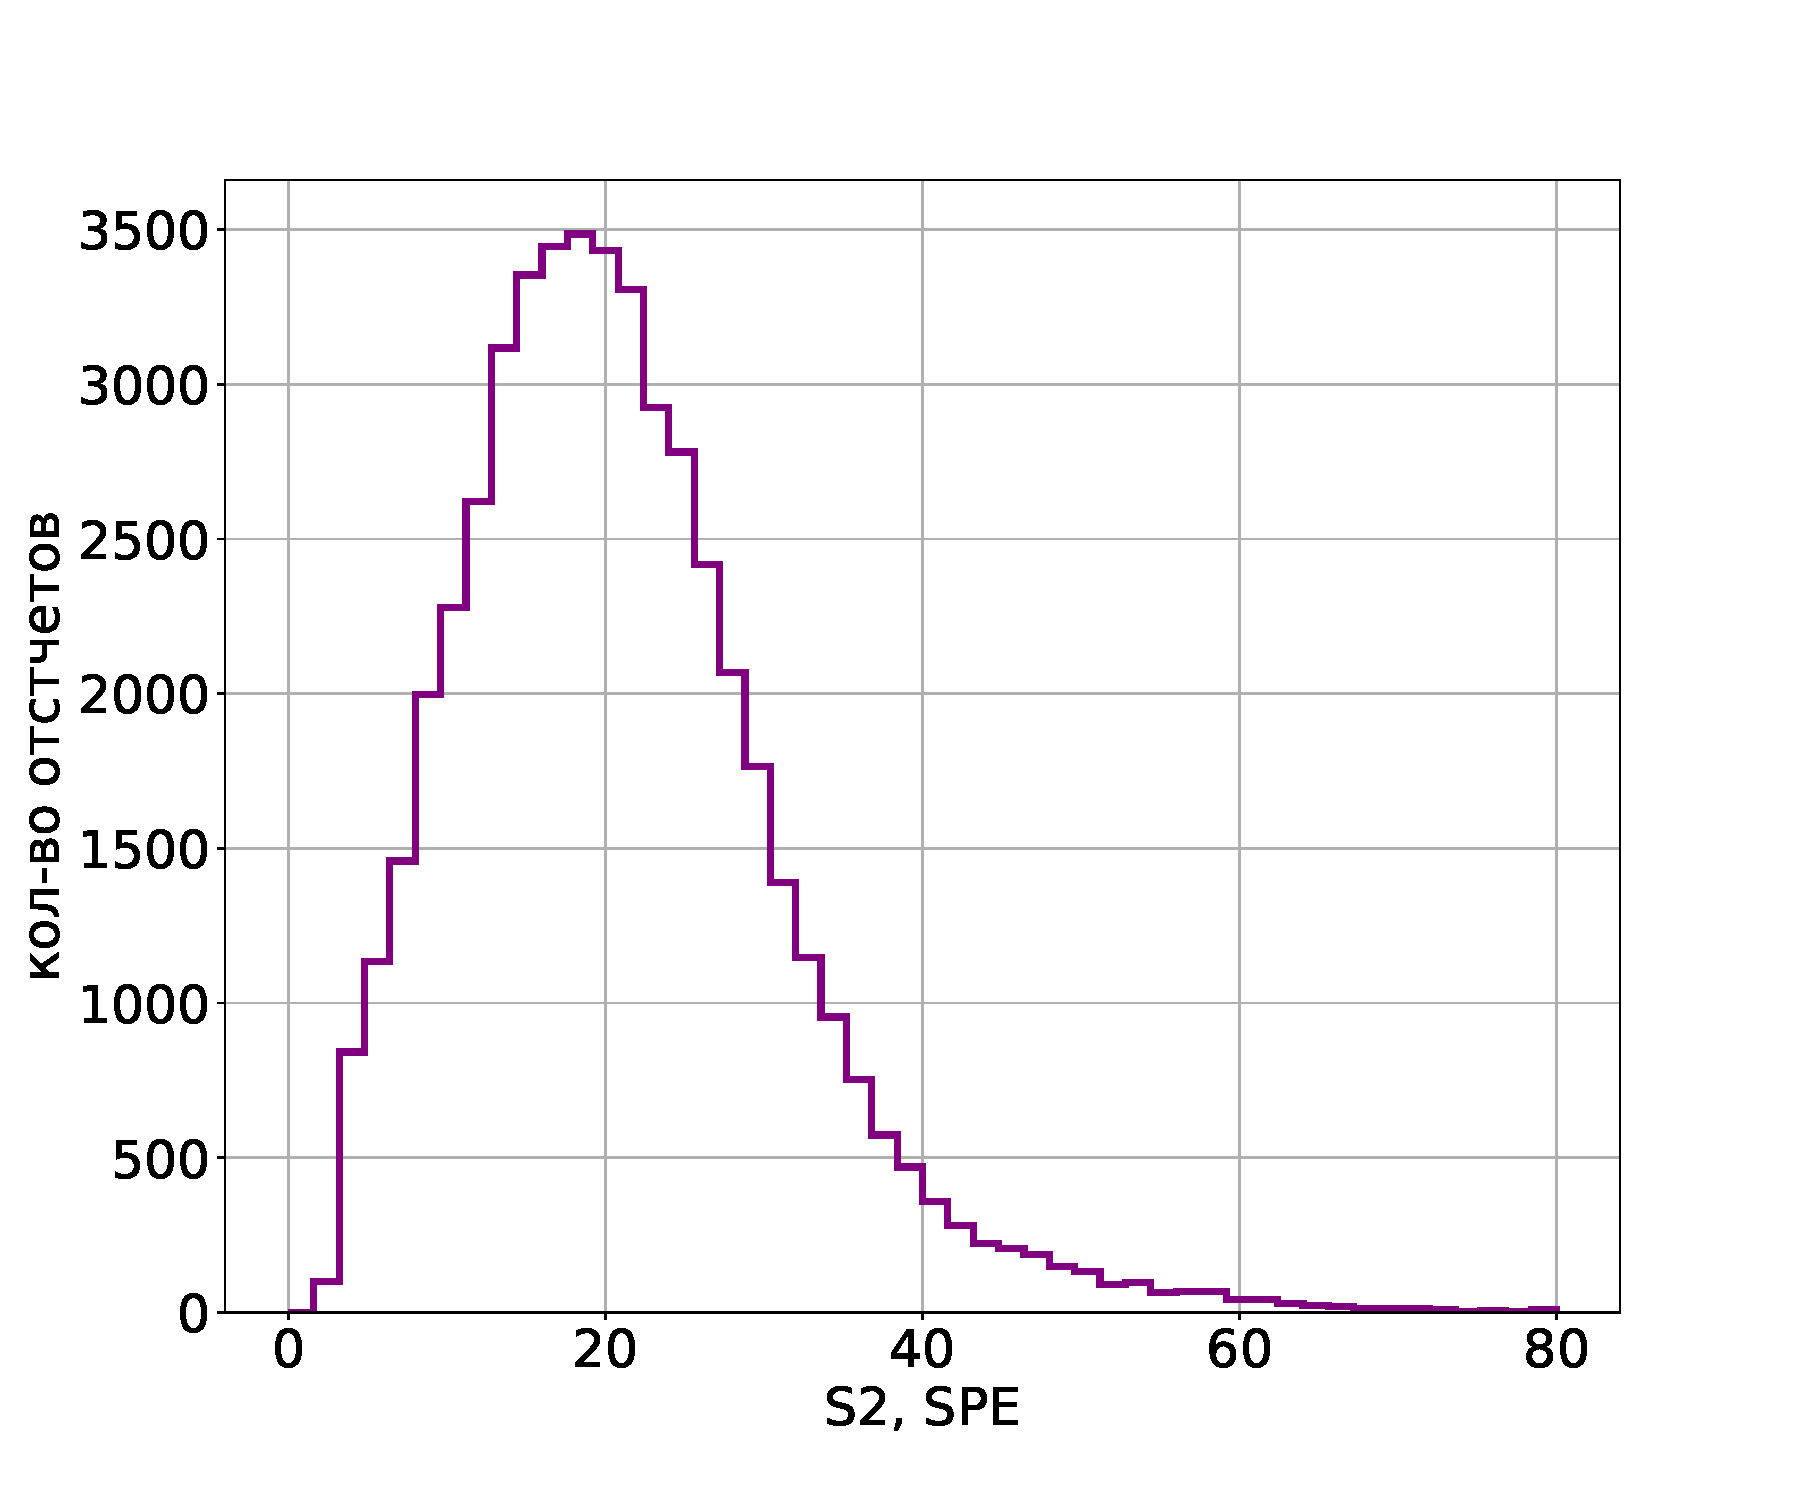
\includegraphics[width=1.0\linewidth]{images/se2022sp.pdf} \\ б)}
  \end{minipage}
  \caption{Распределения S2 в единицах SPE для SE-данных для инженерного сеанса (слева) и сеанса на КАЭС (справа)}
  \label{img:sespesp}  
\end{figure}

\textbf{Раздел 3.5} посвящен вычислению ионизационного выхода и коэффициента экстракции электронов с поверхности жидкого ксенона. 

Расчет ионизационного выхода (ionization yield -- IY) производился путем сравнения величины сигнала электролюминесценции от калибровочных гамма-источников и от одиночных электронов ионизации. Соответственно, для данной процедуры требуется выделение одиночного пика калибровочного гамма-источника. Так как разделение пиков $^{60}$Co возможно только в режиме антикорреляции, был использован пик меньшей энергии и данные SE сигналов. Значение ионизационного выхода рассчитывается по формуле:
\begin{equation}
    IY = k\cdot  \frac{A_{gamma\:source}}{A_{SE}\cdot E} \qquad \left[ \frac{e^-}{keV} \right],
    \label{formula:IY_calc_corr}
\end{equation}
где $A_{gamma\:source}$ и $A_{SE}$ -- положения пиков в фотоэлектронах после процедуры пространственного и энергетического восстановления, a $E$ -- энергия гамма-квантов соответствующего калибровочного источника, k -- поправочный коэффициент, связанный с вычислением площади малых импульсов.

В качестве калибровочного источника, пик от которого присутствует в расчетах, в ЛЭЯФ был использован $^{22}$Na c энергией гамма-квантов 511 кэВ, а при постановке эксперимента на КАЭС -- $^{137}$Cs с энергией гамма-квантов 662 кэВ. Так как расчет коэффициента экстракции электронов важен для предсказания спектра УКРН в детектор, на события был наложен дополнительный отбор на радиус от центра детектора (155 мм для инженерного сеанса и 130 мм для сеанса на КАЭС). Отбор событий, набранных во время сеанса на КАЭС совпадает с отбором, применявшимся для анализа УКРН-событий. Спектры S2 для гамма-калибровочных событий и для SE событий фитировались распределениями Гаусса для получения положений пиков.

Основная идея рассчета коэффициента экстракции электронов состоит в сравнении количества рожденных электронов в месте взаимодействия гамма-кванта с веществом и количества зарегистрированных электронов ионизации по S2. 
Значения величин ионизации для соответствующих энергий, были рассчитаны с использованием программного пакета NEST %версия?. 
\parПолученные значения ионизационного выхода и коэффициента экстракции электронов:
\begin{itemize}
    \item 2019: IY = 15.6$\pm$0.7 e/keV, EEE = 38$\pm$6.1\%
    \item 2022: IY = 12.9$\pm$0.7 e/keV, EEE = 34$\pm$5.9\%
\end{itemize}

Было произведено сравнение полученных значений с измерениями других коллабораций~\cite{Gouschin1978,AprileEEE_2014,Edwards_2018,PhysRevD.99.103024}. Результаты представлены на рисунке \ref{img:EEEworld}. Также на данном рисунке представлен расчет с использованием программного пакета NEST. Результаты, полученные в эксперименте РЭД-100 имеют тенденцию к отличию в большую сторону от общемировых значений. Вероятно, это связано с недостаточной точностью при расчете электрических полей в электролюминесцентном зазоре.

\begin{figure}[ht]
\center{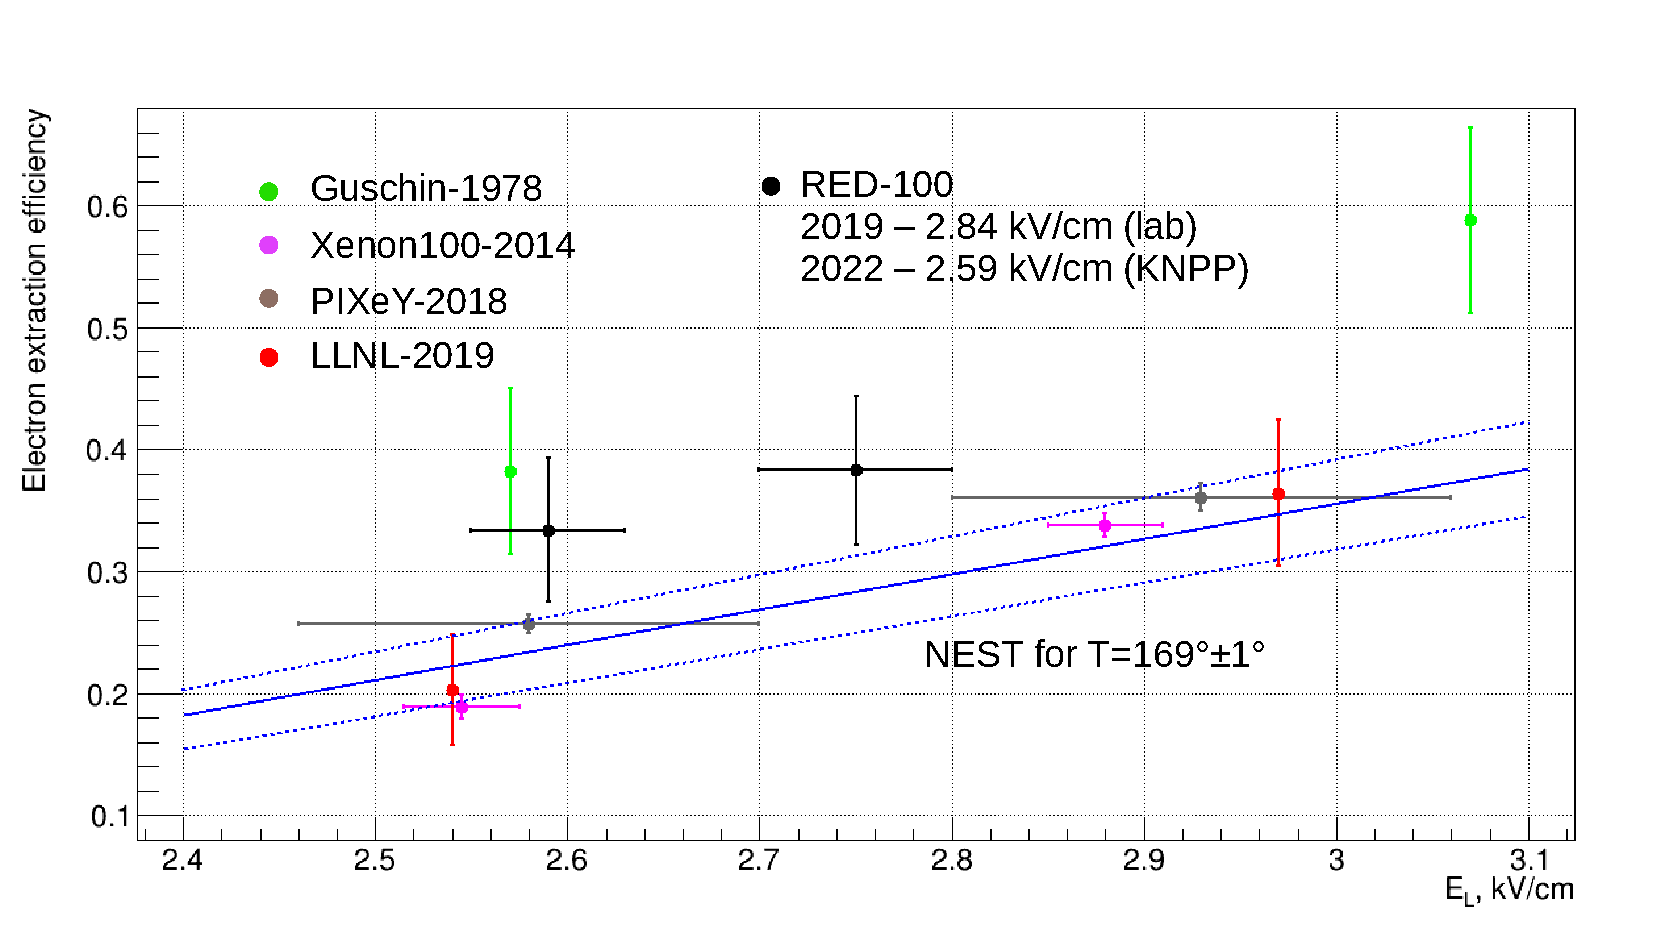
\includegraphics[width=1\linewidth]{images/RED_EEE_With_legend.pdf}}
  \caption{Сравнение результатов измерения ЕЕЕ в эксперименте РЭД-100 и другими коллаборациями, а также резульаты расчета данного коэффициента с использованием программного пакета NEST.}
  \label{img:EEEworld}  
\end{figure}

\underline{\textbf{Четвертая глава}} посвящена анализу физических данных эксперимента РЭД-100 на Калининской АЭС. 

В \textbf{разделе 4.1} описано моделирование ожидаемого сигнала от УКРН. Учитывая известную мощность реактора моделировался энергетический спектр ядер отдачи в GEANT-модели детектора, который далее пересчитывался в спектр, выраженный в электронах ионизации, который далее был скорректирован в соответствии с измеренными потерями при дрейфе и экстракции.

Далее, в соответствии процедурой моделирования временных разверток сигналов были смоделированы события в несколько электронов ионизации согласно полученному спектру. При моделировании использовались LRF, полученные при анализе измерений с гамма-источниками. Также была проведена процедура реконструкции координат и энергии данных событий. Для улучшения соотношения сигнал/шум при дальнейшем анализе к событиям были применены дополнительные отборы по длительности (<5 мкс) и радиусу (<130 мм), совпадающие с отборами для экспериментальных данных. Результирующий спектр восстановленной энергии смоделированных УКРН-событий представлен на рисунке \ref{img:cevnscpectrumspe}. 
\begin{figure}[ht]
\center{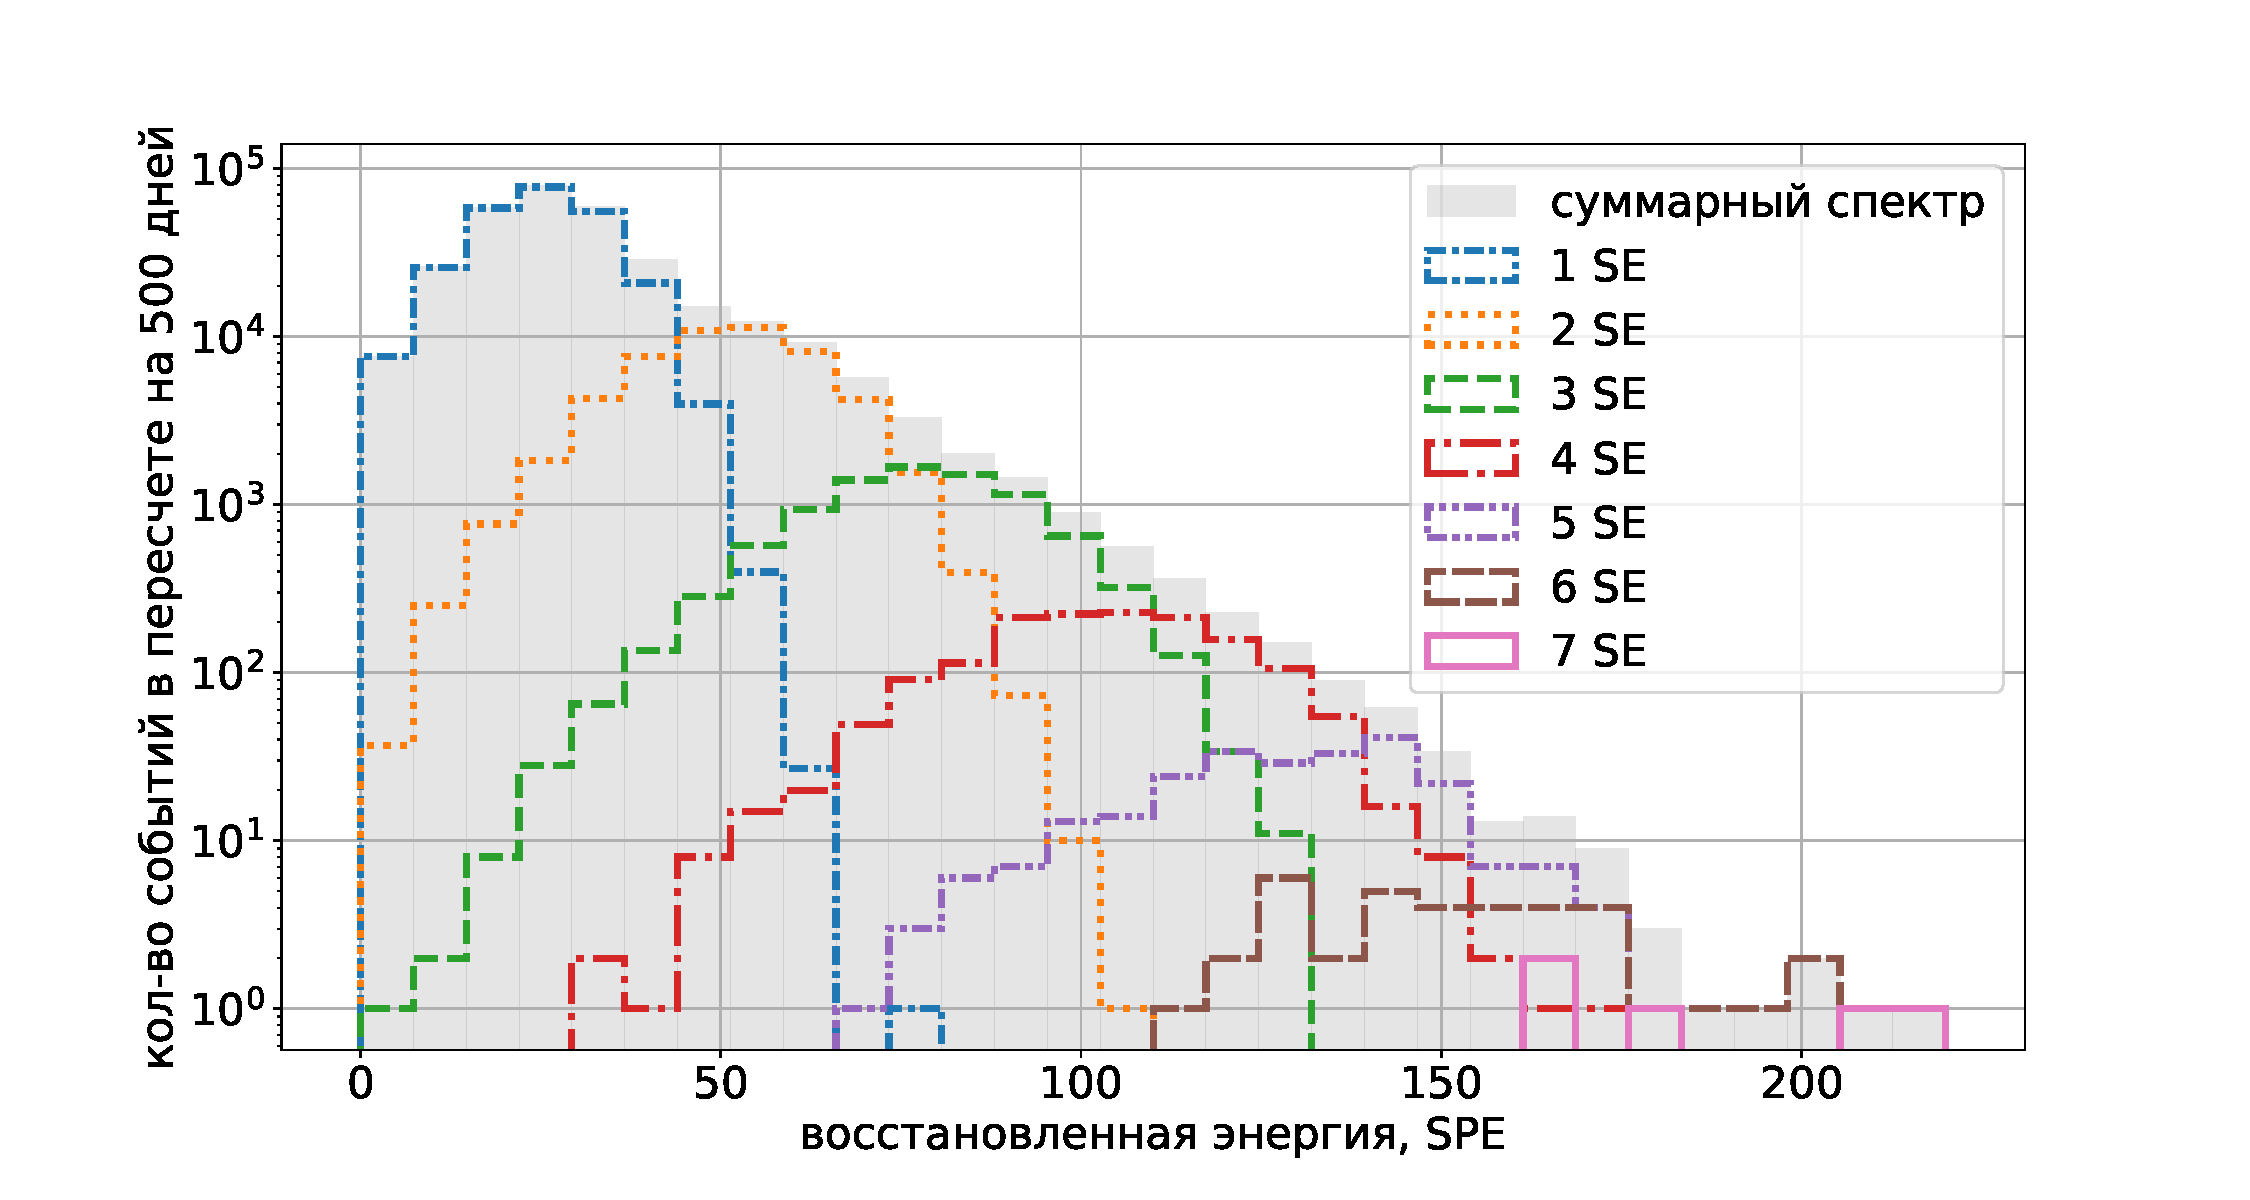
\includegraphics[width=1.0\linewidth]{images/cevnsspectrumSPE.pdf}}
	\caption{Спектр восстановленной энергии смоделирванных УКРН-событий.}
	\label{img:cevnscpectrumspe}
\end{figure}

\textbf{Разделе 4.2} посвящен кластеризации УКРН-подобных событий и отборам. Кластеризация событий в несколько электронов ионизации аналогична процедуре для SE-событий. Отличие заключалось в выборе пороговых значений для отбора импульсов, связанное с изменением SPE-калибровки. Кроме того, на события были наложены дополнительные отборы, описанные в данном разделе, учитывающие форму сигнала и отбор по радиусу (<130 мм). 

Существенную часть фона составляет совпадающие по времени сигналы от одного или нескольких спонтанно возникших электронов ионизации, как показано на рисунке~\ref{img:overlap}.
\begin{figure}[h]
\center{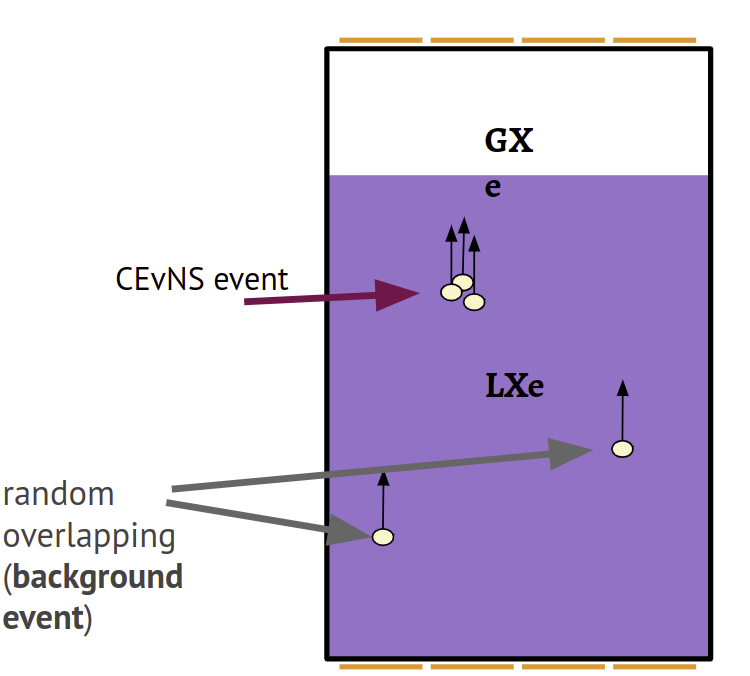
\includegraphics[width=0.5\linewidth]{images/randomoverlap.png}}
	\caption{Иллюстрация механизма возникновения событий совпадения.}
	\label{img:overlap}
\end{figure}

Для борьбы с такими событиями можно использовать идею о том, что точечные события не могут давать множественные вершины на плоскости XY. С целью подавления данной компоненты фона были применены технологии машинного обучения, а именно были разработаны две нейронные сети (перцептрон и сверточная нейронная сеть). Обучение сетей производилось на смоделированных событиях.

Результаты отбора УКРН событий и подавления фона, расчитанные по смоделированным данным приведены в таблицах~\ref{NNeffcevns}~и~\ref{NNeffbckg}. Для дальнейшего анализа отбирались события, идентифицированные обеими сетями как точечные.

\begin{table}[h]
    \centering
    \caption{Эффективности прохождения УКРН-событий для каждой из сетей, расчитанные по смоделированным данным.}  
\begin{tabular}{|c|c|c|c|c|}
\hline Количество SE & 3 & 4 & 5 & 6 \\
\hline сверточная сеть & $0.93$ & $0.96$ & $0.97$ & $0.98$ \\
\hline перцептрон & $0.88$ & $0.91$ & $0.93$ & $0.94$ \\
\hline
\end{tabular}
\label{NNeffcevns}
\end{table}

\begin{table}[h]
    \centering
    \caption{Эффективности подавления фоновых событий для каждой из сетей, расчитанные по смоделированным данным.}  
\begin{tabular}{|c|c|c|c|c|}
\hline Количество SE & 3 & 4 & 5 & 6 \\
\hline сверточная сеть & $0.87$ & $0.87$ & $0.93$ & $0.95$ \\
\hline перцептрон & $0.92$ & $0.93$ & $0.97$ & $0.98$ \\
\hline
\end{tabular}
\label{NNeffbckg}
\end{table}

Энергетический спектр фоновых событий до отборов по радиусу и точечности и после представлен на рисунке~\ref{img:bckgspecrtum}.
\begin{figure}[h]
\center{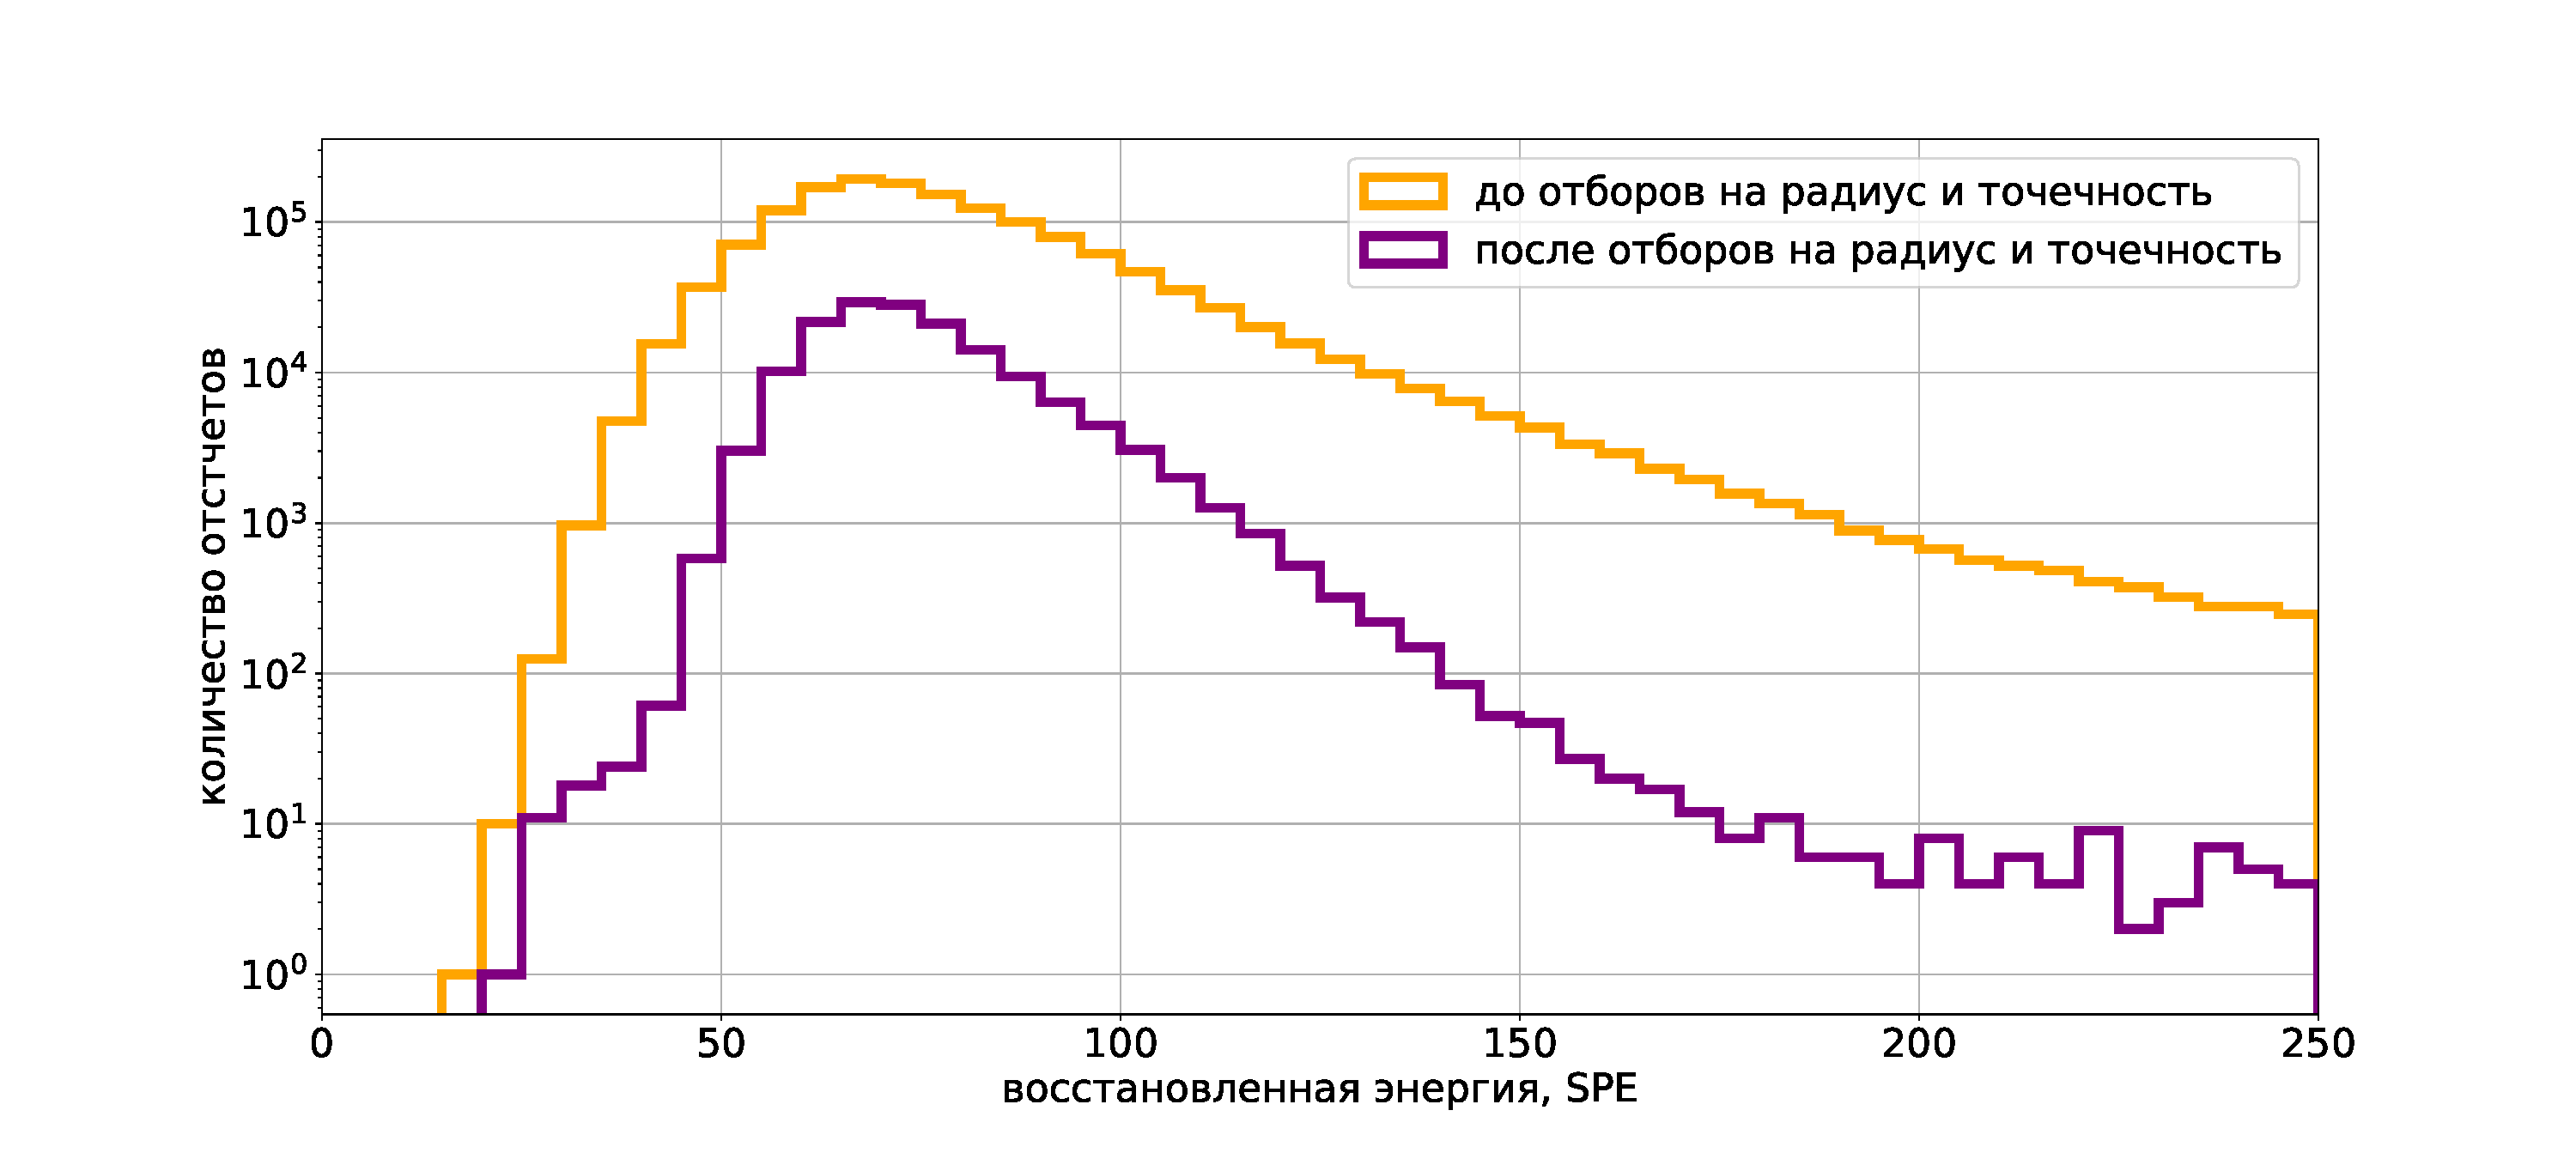
\includegraphics[width=0.8\linewidth]{images/cutsillustration.pdf}}
	\caption{Энергетический спектр фоновых событий до и после отборов по радиусу и точечности}
	\label{img:bckgspecrtum}
\end{figure}

\textbf{Разделе 4.2} посвящен анализу чувствительности детектора к предполагаемому сигналу УКРН. с учетом фонового сигнала. При этом для улучшения результата проводится анализ не только количества событий, но и формы спектра. Также учитывается живое время набора данных с выключенным ($\sim$22 часа) и включенным ($\sim$73 часа) реактором.
Процедура, примененная для анализа чувствительности в данной работе, описана в~\cite{Matt_thesis}. Для анализа был использован трехмерный спектр, где по трем осям были отложены восстановленная энергия, длительность и восстановленный радиус. Общая идея метода состоит в определении количества событий УКРН, которые с определенной пороговой вероятностью не могут быть имитированы случайными флуктуациями фона.

Полученное значение чувствительности ($\approx$37 событий УКРН в день) в $\approx$33 раз превышает предполагаемый уровень сигнала. Ожидаемое количество событий фона и сигнала приведено в таблице \ref{cevnscount}.

\begin{table}[hbt]
    \centering
    \caption{Ожидаемые скорости счета фона и сигнала (в день).}
    
\begin{tabular}{|c|c|c|c|c|}
\hline N e- & 3 & 4 & 5 & 6 \\
\hline bckg & $103 \mathrm{k}$ & $13.6 \mathrm{k}$ & 1268 & 150 \\
\hline CEvNS & $22.7$ & $4.7$ & $0.93$ & $0.19$ \\
\hline
\end{tabular}
\label{cevnscount}
\end{table}

В \underline{\textbf{заключении}} приведены основные результаты работы, которые заключаются в следующем:
%% Согласно ГОСТ Р 7.0.11-2011:
%% 5.3.3 В заключении диссертации излагают итоги выполненного исследования, рекомендации, перспективы дальнейшей разработки темы.
%% 9.2.3 В заключении автореферата диссертации излагают итоги данного исследования, рекомендации и перспективы дальнейшей разработки темы.
Основные результаты данной работы заключаются в следующем:
\begin{enumerate}
  \item Построена детальная оптическая модель детектора РЭД-100. На ее основе построена система моделирования временных разверток сигналов в несколько электронов ионизации в детекторе РЭД-100.
  \item На основе итеративного подхода получены функции распределения светосбора в детекторе РЭД-100 с использованием калибровочных данных с сеансов 2019 и 2022 годов. 
  \item Проведено пространственное восстановление событий в детекторе РЭД-100, на основе результатов было:
  \begin{itemize}
      \item Получено энергетическое разрешение детектора РЭД-100
      \item Получено значение ионизационного выхода
      \item Рассчитан коэффициент экстракции электронов с поверхности жидкого ксенона
  \end{itemize}
  \item Разработаны метод подавления фона неточечных событий на основе нейронных сетей с учетом временных разверток сигналов.
  \item Полученно предсказание сигнала от УКРН в детекторе РЭД-100
  \item Рассчитана чувствительность детектора РЭД-100 к сигналу УКРН
\end{enumerate}

\section*{Публикации автора по теме диссертации}
\begin{enumerate}
    \item First ground-level laboratory test of the two-phase xenon emission detector
RED-100 / D. Akimov [и др.] // Journal of Instrumentation. — 2020. —
февр. — т. 15, No 02. — P02020—P02020. — DOI: https://doi.org/10.1088/1748-0221/15/02/p02020
    \item The RED-100 experiment / D. Akimov [и др.] // Journal of
Instrumentation. — 2022. — нояб. — т. 17, No 11. — T11011. — DOI: 10.
1088/1748- 0221/17/11/T11011. — URL: https://dx.doi.org/10.
1088/1748-0221/17/11/T11011.
\end{enumerate}

%\newpage
%При использовании пакета \verb!biblatex! список публикаций автора по теме
%диссертации формируется в разделе <<\publications>>\ файла
%\verb!../common/characteristic.tex!  при помощи команды \verb!\nocite! 

\ifthenelse{\equal{\thebibliosel}{0}}{% Встроенная реализация с загрузкой файла через движок bibtex8
  \renewcommand{\refname}{\large \authorbibtitle}
  \nocite{*}
  \insertbiblioauthor                          % Подключаем Bib-базы
  \insertbiblioother   % !!! bibtex не умеет работать с несколькими библиографиями !!!
}{% Реализация пакетом biblatex через движок biber
  \insertbiblioauthor                          % Подключаем Bib-базы
  \insertbiblioother
}

         % Содержание автореферата

\end{document}